\documentclass[
  fontsize=10pt,
  twoside=true,
  numbers=noenddot,
  overfullrule=false,
]{kaobook}

\usepackage[english]{babel}
\usepackage[english=american]{csquotes}

\usepackage{kaobiblio}
\addbibresource{main.bib}

\usepackage{mdftheorems}
\usepackage{qmtheorems}

\usepackage{tikz}
\usetikzlibrary{positioning}
\usetikzlibrary{svg.path}
\usetikzlibrary{matrix}

% To set the width of a tikz picture
\usepackage{environ}
\makeatletter
\newsavebox{\measure@tikzpicture}
\NewEnviron{scaletikzpicturetowidth}[1]{%
  \def\tikz@width{#1}%
  \def\tikzscale{1}\begin{lrbox}{\measure@tikzpicture}%
  \BODY
  \end{lrbox}%
  \pgfmathparse{#1/\wd\measure@tikzpicture}%
  \edef\tikzscale{\pgfmathresult}%
  \BODY
}
\makeatother

% Be able to suppress line numbers in listings
\let\origthelstnumber\thelstnumber
\makeatletter
\newcommand*\suppresslinenumbers{%
  \lst@AddToHook{OnNewLine}{%
    \let\thelstnumber\relax%
     \advance\c@lstnumber-\@ne\relax%
    }%
}

\newcommand*\reactivatelinenumbers{%
  \lst@AddToHook{OnNewLine}{%
   \let\thelstnumber\origthelstnumber%
   \advance\c@lstnumber\@ne\relax}%
}
\makeatother

\newcommand{\comment}[1]{\color{gray}#1}

% Reset sidenote counter at chapters
\counterwithin*{sidenote}{chapter}

\begin{document}

\titlehead{A Full Course in Software Engireering}

\title[]{Becoming an Engineer}
\subtitle{From Soup to Nuts: Level 1}

\author[]{Joshua Reyes}

\date{\small\today}

\publishers{Lee Street Publishing}

\frontmatter
% copyright page
\makeatletter
\uppertitleback{\@titlehead} % Header

\lowertitleback{
	\textbf{Disclaimer}\\
	You can edit this page to suit your needs. For instance, here we have a no copyright statement, a colophon and some other information. This page is based on the corresponding page of Ken Arroyo Ohori's thesis, with minimal changes.

	\medskip

	\textbf{No copyright}\\
	\cczero\ This book is released into the public domain using the CC0 code. To the extent possible under law, I waive all copyright and related or neighbouring rights to this work.

	To view a copy of the CC0 code, visit: \\\url{http://creativecommons.org/publicdomain/zero/1.0/}

	\medskip

	\textbf{Colophon} \\
	This document was typeset with the help of \href{https://sourceforge.net/projects/koma-script/}{\KOMAScript} and \href{https://www.latex-project.org/}{\LaTeX} using the \href{https://github.com/fmarotta/kaobook/}{kaobook} class.

	The source code of this book is available at:\\\url{https://github.com/jareyes/qm-companion}

	(You are welcome to contribute!)

	\medskip

	\textbf{Publisher} \\
	First printed in April 2020 by \@publishers
}
\makeatother

% Dedication page
\dedication{``A clever person solves a problem. A wise person avoids it.'' --- Almost certainly not Albert Einstein
\vskip 15pt
For everyone trying to keep afloat.
}

\KOMAoptions{twoside=semi}
\maketitle
\KOMAoptions{twoside=true}

% Preface
\chapter{Preface}

This is the first in a series of short books for people who'd like to get a job in software engineering but who haven't programmed before. These texts are self-paced and build on each other, incorporating skills and concepts used by engineers on the job every day. You're reading the introduction to Level 1.

\section*{Differences from CS 50}
Harvard's CS 50: Introduction to Computer Science is pretty famous. It's a good course, but it's designed for cross-purposes. On the one hand, it's a university course designed for college students who plan to major in computer science. And on the other hand, it is designed to give students who do not plan to major in computer science enough information to build a web app. In my opinion, CS 50 simultaneously does too much and too little to be useful for people who want to make a career in software engineering. It really should dig in deeper into the theory or deeper in the practice.

\section*{Difference from a Programming Bootcamp}
Bootcamps do a good job introducing students to partiular frameworks and specific technologies. And after completing a bootcamp, students have real, living, working completed projects---often web apps---but no real understanding how they work. Web frameworks are plug-and-play. You wire up the built-in components together to do the basic functions in web apps. As soon as projects require a feature that isn't built-in to the framework---as will definitely happen once they get a job---bootcamps stop helping. Bootcamps tend to teach how to use technology, but not how to think and problem like an engineer.

\section*{Our Approach}
This series focuses on thinking and buildling like an engineer does. The content is based on the kinds of problems that engineers experience daily and works through common solutions with an emphasis on transferable skills that apply to all engineering jobs in software---be it web development, mobile app development, backend development, and frontend development.

The series aims to develop core skills and a working intution about programs. After completing this series you will be able to reason about common engineering tasks and problem solve new engineering problems like an software engineer.

We use NodeJS as our language of instruction. NodeJS is a server-side version of JavaScript. We settled on JavaScript for a few reasons. Firstly, JavaScript is the language of the internet. Every browser contains a JavaScript engine. As a result, JavaScript is the most widely supported programming langauge in the entire world. Because you already have a web browser installed on your computer, anyone can start programming without having to set anything up. Because there's nothing initally to set up, you can start programming right away, right now!

Secondly, the syntax and semantics of JavaScript are fairly representative of commonly used programming langauges. Learning JavaScript makes it easy to move to Python or Swift with relatively little extra work.

\section*{Background and Expectations}
This book assumes not previous programming experience. But it does expect that you will read the book carefully, work through the examples, and answer all of the in-text questions, and complete all of the exercises.

Programming is a skill. It is not a set of facts. It is a practice. In order to become a seasoned programmer, you need to program. \emph{A lot.} Watching someone else paint a painting doesn't make you a painter. The only way to become a painter, you need to get your hands dirty, ruin some brushes, and produce a few bad paintings. So, too, with programming. We are going to get real cozy with stack traces, error messages produced by buggy code, and learn to love them.

There is no magic bullet solution. This series will guide you up the mountain of software engineering. But it is a mountain. And it will take time and energy. I know you can do it!

% Table of conents
\etocstandarddisplaystyle % "toc display" as if etoc was not loaded
\etocstandardlines % "toc lines as if etoc was not loaded
\tableofcontents

\mainmatter % Denotes the start of the main document content, resets page numbering and uses arabic numbers
\setchapterstyle{kao} % Choose the default chapter heading style
\setchapterpreamble[u]{\margintoc}
\chapter{Introduction}

Computer science is ths study of what we can compute. Computer scientists try to answer questions like, are there unavoidable limits on the programs we can write? (The answer is \emph{yes}. Some programs are impossible to write no matter what.) And are there unavoidable limits on how slow some programs have to run? (The answer again is yes. We'll see an example of a performance limit later on.) Software engineering is concerned not with whether it is possible to build something---they take the fact that their project can be built for granted---but rather how can the project be built \emph{cheaply}. Software engineers are concerned with how much the project costs, how much time the software takes to run, how much memory it consumes---and, most importantly, whether the whole thing can be shipped to the customer on schedule.

Sucessful programmers need to use a mix of tricks from computer science and software engineering. Generally the two fields grow from one another. Engineers sometiems stumble onto a new, unsolved problem during the course of working on their projects. In the process of completing the project, new computer science is made. Researchers cook up new algorithms to solve outstanding problems in the field. In the process they invent new programming techniques. Those new techniques make it back to the engineers, who then apply them in new projects. And so the cycle goes on and on. What computer scientists and software engineers do aren't that different. They approach similar problems with different perspectives. To be a sucessful programmer, you will sometimes want to think like a computer scientist and sometimes like a software engineer. Fortunately, both perspectives come from the same underlying idea of computation, which can be drawn very neatly in a diagram---the \emph{fundamental diagram}.

\section{The Fundamental Diagram}
The \textbf{Fundamental Diagram} is at the heart of everything software engineers and computer scientists do.\sidenote{Full disclaimer: I might be the only person who calls this the Fundamental Diagram. But everyone should. Like reading, this diagram is fundamental.} As a programmer, you'll get to know this picture very well. It shows up in just about every concept you'll ever encounter---from the very big, to the obnoxiously small.

\begin{figure}[h]
  \begin{scaletikzpicturetowidth}{\textwidth}
  \begin{tikzpicture}[scale=\tikzscale, node distance=3cm, color=cyan, font=\sffamily\small]

    \node[draw, thick, fill=cyan!20, minimum size=2em, inner sep=1em] (transformer) {Transformer};
    \node (inputs) [left of=transformer] {Inputs};
    \node (outputs) [right of=transformer] {Outputs};

    \draw[->, thick, shorten >= 1em, shorten <= 0.25em] (inputs) -- (transformer);
    \draw[->, thick, shorten >= 0.25em, shorten <= 0.5em] (transformer) -- (outputs);

  \end{tikzpicture}
\end{scaletikzpicturetowidth}

  \caption{\label{fig:intro-fundemental-diagram} The Fundamental Diagram of computer science and software engineering in all its glory. It describes just about everything a programmer could possibly do.}
\end{figure}

Fortunately, the diagram doesn't have many parts. There are just three: the inputs, the outputs, and the transformer. The transformer takes in \emph{inputs} and \emph{transforms} them into \emph{outputs}. That's it. As a programmer, you will write software that turns specific inputs into particular outputs to accomplsh a given task. If that description sounds vague, that's because it is. Let's look at a few examples to see the Fundamental Diagram in action to get a better idea of what's going on.

\paragraph{Example (Question and Answer)} A lot of human interaction follows the input-transformer-output pattern. Questions and answers can be modeled by the fundamental diagram pretty easily. For example, ``What's your favorite color?''\sidenote{The answer is orange. Well, it is if I am the transformer being asked. You might come up with a different but correct answer. Different transformers can give different answers to the same question.} But what is the transformer in this case? The transformer is the person who gives the answer to the question; she listens to a question asked by somebody else, processes what it means, and then produces an answer. For historical reasons---think ancient Greek history---sometimes the role of the transformer in a Q\&A session is called an \emph{oracle}.

\begin{figure}[h]
  \begin{scaletikzpicturetowidth}{\textwidth}
  \begin{tikzpicture}[scale=\tikzscale, node distance=3cm, color=cyan, font=\sffamily\small]

    \node (inputs) {Question};
    \node (question) [below=0em of inputs] {What is your favorite color?};

    \node[draw, thick, fill=cyan!20, minimum size=2em, inner sep=1em] (transformer) [right of=inputs] {Oracle};
    \draw[->, thick, shorten >= 1em, shorten <= 0.25em] (inputs) -- (transformer);

    \node (outputs) [right of=transformer] {Answer};
    \node (answer) [below=0em of outputs] {Orange.};
    \draw[->, thick, shorten >= 0.25em, shorten <= 0.5em] (transformer) -- (outputs);

  \end{tikzpicture}
\end{scaletikzpicturetowidth}

  \caption{\label{fig:intro-example-question-answer} Fundamental diagram for a question, oracle, and answer.}
\end{figure}

\paragraph{Example (Request and Response)}The same can be said of slightly different kind of speech act called a \emph{request}. People make requests all the time. ``Can you close the door, please?'' ``May I have the lobster sandwich and a raspberry lime rickey?'' ``That'll be \$49.99, please.'' Each of these statements intend to turn simple words into actions that produce some physical effect---producing closed door, a lobster sandwich and a raspberry lime rickey, or money totaling \$49.99.

\begin{question}
  \label{question:intro-transformers}
  Identify the inputs, outputs, and transformers for the requests above.
\end{question}

\begin{question}
  Draw the fundamental diagrams for each of the requests above.
\end{question}

On the web, requests are ubiquitous. When you open a web browser and type in the address of a web page, the web browser makes a formal request to the machine located at that address. \sidenote{In the same way individual people have street addresses---like Sirius Black, who resided at 12 Grimmauld Place, London---computers have internet addresses, too. These computers are called \emph{web servers}. Like the computer which resides at the address \texttt{www.dafk.net}.\vskip 5pt Individual web pages reside on web servers. For example, the webapge \texttt{what} resides on the computer with the address \texttt{www.darfk.net}. Its full address is \texttt{www.darfk.net/what}.} The terminology for the actors in a web request comes from the restaurant industry. At restaurants, clients make requests to people called servers, who fulfill their clients' requests (usually with the help of many other people who are not client-facing).

This pattern of request and response is exactly how the world wide web works. The piece of software that initiates the request is called the \emph{client}. Because this is the software that human users can see, people sometimes say client technology is \emph{front end} technology. The software that receives, processes, and sends back a response to the client is called the \emph{server}. The server is not something that human users interact with directly. We don't get to see what the server is doing, only the response that it produced. This is a lot like how clients at a restaurant don't get to interact with the kitchen directly. Instead they get to experience the finished product---but they don't get know how the sausage is made, so to speak. Because the server's work to transform a request into a full web page response is opaque to the user, we say that servers a \emph{back end} technology.

\begin{figure}[h]
  \begin{scaletikzpicturetowidth}{\textwidth}
  \begin{tikzpicture}[scale=\tikzscale, node distance=3cm, color=cyan, font=\sffamily\small]

    \node (inputs) {Request};
    \node[minimum size=2em, inner sep=1em] (question) [below=0em of inputs] {\texttt{www.dafk.com/what}};

    \node[draw, thick, fill=cyan!20, minimum size=2em, inner sep=1em] (transformer) [right of=inputs] {Server};
    \node (server) [below=0em of transformer] {\texttt{www.dafk.com}};
    \draw[->, thick, shorten >= 1em, shorten <= 0.25em] (inputs) -- (transformer);

    \node[minimum size=2em, inner sep=1em] (outputs) [right of=transformer] {Response};
    \node (response) [below=0em of outputs] {Contents of \texttt{what}};
    \draw[->, thick, shorten >= 0.25em, shorten <= 0.5em] (transformer) -- (outputs);

  \end{tikzpicture}
\end{scaletikzpicturetowidth}

  \caption{\label{fig:intro-example-request-response} Fundamental diagram for a request, server, and response.}
\end{figure}

The client-server architecture, like the fundamental diagram, is deceptively simple and yet it powers the whole of the internet.\sidenote{Software engineers call the organization of data flows an \emph{architecture}. In this case, the flow of information is the request from the client to the server and the response from server to client.} Web programming is a specialized collection of technologies, many of which we'll encounter in this series. When you're bushwacking the jargon and buzzwords of the web technology jungle, stop and remember Figure \ref{fig:intro-example-request-response}: just two arrows and a box in the middle. Almost all of the latest and greatest technologies are just fancy ways to request some piece of data from a server. Always keep this picture in mind.

\paragraph{Example (Making Ice Cream)} Recipes are hands-down the tastiest kinds of transformers.Recipes explain how to transform ingredients into prepared dishes. Here's one I like because it's quick, easy, and the result is something near and dear to my heart: ice cream.

\begin{marginfigure}
  \begin{scaletikzpicturetowidth}{\textwidth}
  \begin{tikzpicture}[scale=\tikzscale, color=cyan, font=\sffamily\footnotesize]
    \node (input) at (0,0) {};
    \node[draw, thick, fill=cyan!20, minimum size=1em, inner sep=0.5em] (transformer) at (1,0) {Recipe};
    \node (output) at (2,0) {};

  % https://thenounproject.com/search/?q=milk&i=1577815
  % Milk by Wawan Hermawan from the Noun Project
    % \draw[fill=cyan, rotate=180, scale=0.15] (0,0) svg "M50.5283203,62.3232422c-0.4343262-2.0397949-2.357605-3.3642578-4.3845215-3.1366577   c0.6894531-0.8180542,1.1194458-1.965271,0.9138184-3.4907837c-0.1113281-0.8208008-0.8583984-1.3964844-1.6865234-1.2866211   c-0.8212891,0.1108398-1.3964844,0.8657227-1.2861328,1.6870117c0.119812,0.8925171-0.2557983,1.3293457-0.717041,1.5389404   c-0.9266357-0.5111084-1.9899902-0.8035889-3.1208496-0.8035889c-1.1310425,0-2.194519,0.2926025-3.1212769,0.803833   c-0.4609375-0.2095337-0.8362427-0.6469116-0.7166138-1.5391846c0.1103516-0.8212891-0.4648438-1.5761719-1.2861328-1.6870117   c-0.8300781-0.109375-1.5761719,0.4658203-1.6865234,1.2866211c-0.2055054,1.5245361,0.2238159,2.6713257,0.9122925,3.4892578   c-0.9240723-0.1054688-1.8487549,0.0901489-2.638855,0.6030273c-0.9013672,0.5844727-1.5205078,1.4848633-1.7441406,2.5351563   c0,0,0,0,0,0.0004883c-0.0957031,0.4482422-0.109375,0.9208984-0.0390625,1.4038086   c0.0625,0.4350586,0.3125,0.8208008,0.6845703,1.0556641c0.4121094,0.2597656,0.8486328,0.4404297,1.2978516,0.5361328   c0.28125,0.0595703,0.5644531,0.0893555,0.8457031,0.0893555c0.4030762,0,0.8010864-0.0646362,1.1846924-0.1845093   c0.2687988,1.8319702,0.8359985,4.2652588,1.6209717,6.3978882c0.2167969,0.5898438,0.7783203,0.9819336,1.4072266,0.9819336   h6.5576172c0.6289063,0,1.1904297-0.3920898,1.4072266-0.9819336c0.7855225-2.133606,1.3529053-4.5665894,1.6218262-6.3979492   c0.383606,0.119873,0.7816772,0.1845703,1.1848145,0.1845703c0.28125,0,0.5644531-0.0297852,0.8457031-0.0893555   c0.4462891-0.0952148,0.8818359-0.2753906,1.2958984-0.534668c0.3730469-0.234375,0.6240234-0.6210938,0.6865234-1.0571289   c0.0703125-0.4829102,0.0566406-0.9555664-0.0390625-1.4038086C50.5283203,62.3232422,50.5283203,62.3232422,50.5283203,62.3232422   z M42.4560547,69.6040039h-4.4189453c-0.8242188-2.5600586-1.2744141-5.2426758-1.2744141-6.2880859   c0-1.9213867,1.5634766-3.484375,3.484375-3.484375s3.484375,1.5629883,3.484375,3.484375   C43.7314453,64.3603516,43.2802734,67.0424805,42.4560547,69.6040039z";

    \draw[fill=cyan, rotate=180, shift={(-0.15,-0.22)}] svg[scale=0.13pt] "M24.7421875,96h27.2958984h3.7138672H74.5c0.828125,0,1.5-0.6713867,1.5-1.5v-62   c0-0.0164185-0.0042725-0.0316772-0.0048218-0.0479736c-0.001709-0.053772-0.008667-0.105957-0.0159302-0.1582031   c-0.0065918-0.0474243-0.0126953-0.0948486-0.0239258-0.1419678c-0.0107422-0.0448608-0.026001-0.0877075-0.0406494-0.1308594   c-0.0175171-0.0516357-0.0355225-0.1032104-0.059082-0.1536865c-0.0066528-0.0143433-0.0095825-0.0293579-0.0167236-0.0435791   l-8.9316406-17.6810303V5.5c0-0.8286133-0.671875-1.5-1.5-1.5H34.5927734c-0.828125,0-1.5,0.6713867-1.5,1.5v8.267334   c-0.0049438,0.0088501-0.0127563,0.0151978-0.0175781,0.0241699l-9.6494141,18   c-0.0020752,0.0038452-0.0025024,0.0081177-0.0045166,0.0119629C23.31073,32.0124512,23.2421875,32.2470703,23.2421875,32.5v62   C23.2421875,95.3286133,23.9140625,96,24.7421875,96z M52.0380859,93H26.2421875V34h25.7958984h2.2138672v59H52.0380859z M73,93   H57.2519531V34H73V93z M72.0617676,31H58.2639771l7.1038208-13.2514038L72.0617676,31z M36.0927734,7h27.8144531v6H36.0927734V7z    M35.2949219,16h27.6064453l-8.0410156,15h-2.8222656H27.2539063L35.2949219,16z";

    % https://thenounproject.com/search/?q=ice%20cream%20cone&i=1422432
    % Ice Cream by Landan Lloyd from the Noun Project
    \draw[fill=cyan, rotate=180, shift={(-2.40,-0.35)}] svg[scale=0.2pt] "M64.71,53a5.12,5.12,0,0,0-.78-2.71,13.46,13.46,0,0,0-.23-5.49,5.71,5.71,0,0,0,.45-5.44c0-.06,0-.11,0-.16a12.7,12.7,0,0,0-3-9.58A5,5,0,0,0,61.36,28a5.15,5.15,0,0,0-1-2.69,10.74,10.74,0,0,0-10.61-8.94l-.67,0A10.74,10.74,0,0,0,39,27.52a5.45,5.45,0,0,0-.33,2.27,5.34,5.34,0,0,0,.52,2,12,12,0,0,0-1.31,3.86,5.87,5.87,0,0,0-1,2.71,5.71,5.71,0,0,0,.72,3.47,13.88,13.88,0,0,0-1.47,6.25v.39a5.79,5.79,0,0,0,2,7.92l7.66,23.94a4.5,4.5,0,0,0,8.64,0l7.29-22.67A5.13,5.13,0,0,0,64.71,53Zm-3.6-4.9a11.06,11.06,0,0,1-.45,3.07A2.12,2.12,0,0,1,61.71,53a2,2,0,0,1,0,.25h0a3.61,3.61,0,0,1-.08.38h0a1.43,1.43,0,0,1-.14.34v0a1.81,1.81,0,0,1-.19.29l0,.05-.21.22-.09.07a1.66,1.66,0,0,1-.21.16l-.15.08-.19.1-.23.07-.15,0a1.84,1.84,0,0,1-.41,0l-.26,0h0a2.11,2.11,0,0,1-1.83-1.79h0a2.77,2.77,0,0,1-.71-.1,2,2,0,0,1-1.84,1.21,2,2,0,0,1-1.38-.56,2.77,2.77,0,0,1-4.18-.19,1.16,1.16,0,0,1-.9.43,1.18,1.18,0,0,1-1-.52,3.08,3.08,0,0,1-1.57.43,3.16,3.16,0,0,1-1.19-.24,1.72,1.72,0,0,1-3.19.47,3.13,3.13,0,0,1-.44,0,3,3,0,0,1-.52,0h0a3,3,0,0,1-.72-.24l-.08,0a2.6,2.6,0,0,1-.59-.41h0a3,3,0,0,1-.8-1.34h0a2.84,2.84,0,0,1-.1-.72,2.77,2.77,0,0,1,.91-2.06,9.5,9.5,0,0,1-.09-1.31,11.05,11.05,0,0,1,.75-4A5.59,5.59,0,0,0,42,44.8a4.54,4.54,0,0,0,.63,0,5.76,5.76,0,0,0,2.4-.53,5.81,5.81,0,0,0,1.37.32l.66,0a4,4,0,0,0,.49,0,5.77,5.77,0,0,0,3.83,2.06c.21,0,.43,0,.64,0a5.68,5.68,0,0,0,2.37-.51l.51.09.45,0a5.8,5.8,0,0,0,2.85,1.13l.63,0a5.81,5.81,0,0,0,2.21-.44A9.28,9.28,0,0,1,61.11,48.11ZM61.62,42a2.39,2.39,0,0,1-.14.6l-.06.16a2.32,2.32,0,0,1-.22.41l-.07.12a2.89,2.89,0,0,1-.91.83h0a2.82,2.82,0,0,1-1.38.37h-.31A2.84,2.84,0,0,1,56.37,43a1.6,1.6,0,0,1-1,.31h-.18a1.62,1.62,0,0,1-1.08-.57,2.79,2.79,0,0,1-2.12,1h-.31a2.8,2.8,0,0,1-2.48-3,3,3,0,0,1-2.17.92h-.33a3.07,3.07,0,0,1-1.86-.93,2.84,2.84,0,0,1-2.22,1.12h0l-.3,0a2.93,2.93,0,0,1-.94-.28h0l-.31-.18-.07,0a3,3,0,0,1-.76-.8v0A2.78,2.78,0,0,1,39.84,39a2.43,2.43,0,0,1,0-.27,2.82,2.82,0,0,1,.93-1.78c0-.09,0-.18,0-.27a9.45,9.45,0,0,1,.59-2.45,5.55,5.55,0,0,0,2.85.8h.34a5.42,5.42,0,0,0,2.3-.65,6.33,6.33,0,0,0,2,.32h.38a6.34,6.34,0,0,0,3.49-1.32h.34a5.36,5.36,0,0,0,1.12-.19,5.18,5.18,0,0,0,2,.41h.32a5.09,5.09,0,0,0,3-1.21,9.61,9.61,0,0,1,1.7,6.55c0,.36-.11.7-.18,1A2.78,2.78,0,0,1,61.62,42ZM42,27.56a7.71,7.71,0,0,1,7.28-8.13l.49,0a7.72,7.72,0,0,1,7.74,7.2s0,0,0,0a2.3,2.3,0,0,1,.52.6h0a3.55,3.55,0,0,1,.21.44s0,0,0,0a2.28,2.28,0,0,1,.1.52,2.32,2.32,0,0,1,0,.53l0,.13a2.7,2.7,0,0,1-.14.4.2.2,0,0,0,0,.08,2.21,2.21,0,0,1-.72.8h0a2.09,2.09,0,0,1-1.08.37h-.13a2.2,2.2,0,0,1-1.76-.9,2.4,2.4,0,0,1-1.54.68h-.14a2.5,2.5,0,0,1-1.06-.25,3.37,3.37,0,0,1-2.63,1.57h-.2a3.33,3.33,0,0,1-2.38-1A2.53,2.53,0,0,1,44.39,32h-.16a2.57,2.57,0,0,1-1.29-.35h0a2.63,2.63,0,0,1-.85-.81L42,30.74a3.11,3.11,0,0,1-.2-.41.78.78,0,0,0,0-.14,2.3,2.3,0,0,1-.1-1,2.14,2.14,0,0,1,.06-.35,2.66,2.66,0,0,1,.35-.83C42.07,27.88,42,27.73,42,27.56ZM51.5,79.49a1.51,1.51,0,0,1-2.9,0L41.71,57.93a4.63,4.63,0,0,0,1.34.21,4.72,4.72,0,0,0,3-1.12,5.49,5.49,0,0,0,1.07-.13,4.13,4.13,0,0,0,1.3.22l.42,0a5.81,5.81,0,0,0,4.87.2,5.06,5.06,0,0,0,1.17.14,5.18,5.18,0,0,0,1.67-.28,5.2,5.2,0,0,0,1.82.83Z";

    \draw[->, thick, shorten >= 0.25em, shorten <= 0.25em] (input) -- (transformer);
    \draw[->, thick, shorten >= 0.25em, shorten <= 0.25em] (transformer) -- (output);


  \end{tikzpicture}
\end{scaletikzpicturetowidth}

  \caption{\label{fig:intro-example-ice-cream} Total preparation time is about 15 minutes plus a 20 minutes soft freeze in the ice cream maker followed by an overnight hard freeze in the freezer.\vskip 5pt Milk by Wawan Hermawan and ice cream by Landan Lloyd from the Noun Project.}
\end{marginfigure}

Up until now, each transformer we've described takes exactly one input and produces a single output. Here is our first example of a transformer that takes multiple inputs to produce its output. It is not uncommon for a transformer to take multiple inputs. There are very few recipes that require just a single ingredient. So, too, programs often need to use combine multiple inputs to generate a desired output.

Let's look at the process to transform a few ingredients into ice cream in some detail. Below is a kind of step-by-step list of instructions that transform the input ingredients milk, cream, sugar, and salt, into ice cream. Each step goes on its own line. As a general rule, steps should be kept as simple as possible. Complex steps should be broken up into multiple, simpler steps. This strategy makes it easier for the person preparing the recipe to understand and execute. The programs we write to transform inputs into outputs will have a very similar character.

\suppresslinenumbers
\begin{lstlisting}[caption={\label{listing:intro-ice-cream} Ice cream transformer. It's as short as it is sweet.}, escapeinside=$$, firstnumber=0]
$\textbf{Inputs:}$ 1 c. whole milk
        2 c. heavy cream
        2/3 c. sugar
        1/2 tsp. Kosher salt

$\textbf{Output:}$ Sweet cream ice cream
$\reactivatelinenumbers$
Place the milk, heavy cream, sugar, and salt in a bowl.
Mix until the sugar has completely dissolved.
Pour the ice cream base into an ice cream maker.
Run the machine until the base mixture firms up.
Transfer the cold cream into a sealed container.
Chill the container in a freezer overnight.
\end{lstlisting}

Did you notice that our great big ice cream transformer is made up of three smaller input-output transformers? The first one decribed on lines 1--2. It turns the input ingredients into a liquid base mixture. The next one on lines 3--4 takes as input the base mixture and outputs a cold cream. While cold cream is delicious, it melts extremely rapidly. And so the recipe finishes with the transformer on lines 5--6, which takes as input the cold cream and freezes it until to produce bona fide ice cream.

\begin{figure*}[h]
  \begin{scaletikzpicturetowidth}{\textwidth}
  \begin{tikzpicture}[scale=\tikzscale, color=cyan, node distance=3cm, font=\sffamily\small]

    % liquid base transformer
    \node (ingredients) {Ingredients};
    \node[draw, thick, fill=cyan!20, minimum size=2em, inner sep=1em] (mixer) [right of=ingredients] {Combine};
    \draw[->, thick, shorten >= 1em, shorten <= 0.25em] (ingredients) -- (mixer);

    \node (base) [right of=mixer] {Liquid Base};
    \draw[->, thick, shorten >= 0.25em, shorten <= 0.25em] (mixer) -- (base);

    % cold cream transformer
    \node[draw, thick, fill=cyan!20, minimum size=2em, inner sep=1em] (maker) [below=1cm of base] {Soft Freeze};
    \draw[->, thick, shorten >= 0.25em, shorten <= 0.5em] (base) -- (maker);

    \node (cold cream) [right of=maker] {Cold Cream};
    \draw[->, thick, shorten >= 0.25em, shorten <= 0.5em] (maker) -- (cold cream);

    % ice cream transformer
    \node[draw, thick, fill=cyan!20, minimum size=2em, inner sep=1em] (freezer) [below=1cm of cold cream] {Hard Freeze};
    \draw[->, thick, shorten >= 0.25em, shorten <= 0.5em] (cold cream) -- (freezer);

    \node (ice cream) [right of=freezer] {Ice Cream};
    \draw[->, thick, shorten >= 0.25em, shorten <= 0.5em] (freezer) -- (ice cream);
  \end{tikzpicture}
\end{scaletikzpicturetowidth}

  \caption{\label{fig:intro-example-ice-cream-pipeline} The steps inside transformers are often simpler transformers. The transfromation that produces ice cream from ingredients is made up of three successive transformers. The output of one transformer is the input to the next transformer.}
\end{figure*}

Figure \ref{fig:intro-example-ice-cream-pipeline} illustrates that old saying, ``One transformer's output is another transformer's input.'' And that is the real power of the fundamental diagram. You can chain copies of it together to produce more and more complicated flows of inputs and outputs. In this case, we chained together three transformers in the simplest way possible, in a line, one after the other. The \emph{pipeline} pattern is very common in software architecture. In fact, many of the applications in ``big data'' reduce to pipelines of transformers, no different conceptually to the ice cream pipeline above. When we work with command line tools, we will meet the pipe operator that feeds the output of one program as the input to another.\sidenote{The pipe operator notated by the symbol `\texttt{|}`. It's that shift character on the backslash key. Now go lay some pipe!} It acts like a pipe for the information to flow through. Hence the name \emph{pipe}.

\begin{question}
  In the style of Listing \ref{listing:intro-ice-cream}, write the inputs, outputs, and steps to create a grilled cheese sandwich.
\end{question}

\begin{question}
  Draw a fundamental diagram for your grilled cheese listing.
\end{question}

\begin{question}
  Come up with three more examples that can be modeled by the fundamental diagram.
\end{question}

\section{Programs}
You will use a text editor to write your programs, because programs are a kind of written text. You can think of them as a sort of genre. Programs follow the rules and conventions of their genre---the same as a sales brochure or novel do. And like any other work of literature, can be judged on any number of dimensions---readability, structure, flow, rhythm---so, too, can the text (code) of an individual program be judged sloppy or sublime. There are a lot of strong opinions about how to organize code. And religious wars about what a good program looks like break out all the time. And just as good writing takes lots of practice and revision, so does writing a good program.

Writing a program is an iterative process, with many drafts, edits, and restructuring. The practice of editing a program is so important that it has been given a special name, \emph{refactoring}. Refactoring is the process of restructuring code in a program to improve it somehow. Often the aim of refactoring is understandability. Remember, programs are for human-readers, not computers. \marginnote{Other programmers include \emph{you} in the future. You think you'll remember what you were thinking when you wrote that obtuse line of code, but I promise you, you will not.} So you should go to great pains to make your code legible and digestable to other programmers. Other goals include troubleshootability, extensibility, and performance.

Refactoring isn't separate from programming. It's part of writing, drafting, and improving every program you write. Refactoring projects can be as small as changing a variable name, or as large as a full-scale project rewrite. Usually they range somewhere in between. Refactoring is an essential skill. We will refactor many of the programs we write in this book because we refactor many of the programs we write on the job.

Most genres contain subgenres. Within the novel you find mystery novels, romance novels, travel novels, and other that cross and combine subgenres. Programs constitute a large genre. Quite naturally, the field has split in many kinds of programming: systems programming, graphics programming, web application programming, game programming, scientific programming, etc. All of kinds of programming, however, rely on foundational concepts and common techniques.

Genre transcends language. Novels and sales brochures can be written in any language. And the same general rules apply whether written in English or Swedish. Programs can be written in a variety programming languages. Most programming languages are designed for human readers and writers. The machines, which execute the instructions written in code, however, speak their own \emph{machine languages}. And the contents of the text files that programmers produce need to be converted into directives that can be carried out reliably and directly on hardware. There are two special kinds of programs that perform the translation from a source programming language to machine language: compilers and interpreters. The difference is that compilers take in a full program and convert it all at once. Interpreters take in one statement of programming at a time and convert on the fly. (Much the same difference between translating a book---the compiler---and what someone is saying in real-time---an interpreter.)

\section{Compilers} One of the most important transformer in programming is type of program called a \emph{compiler}. Compilers translate programs from one language into another---specifically, from a \emph{source language} that humans can read, write, and understand to a \emph{target language} that computers can interpret and execute.

\begin{figure}[h]
  \begin{scaletikzpicturetowidth}{\textwidth}
  \begin{tikzpicture}[scale=\tikzscale, node distance=3cm, color=cyan, font=\sffamily\small]

    \node (inputs) {Program Instructions};
    \node (question) [below=0em of inputs] {JavaScript/Python/etc.};

    \node[draw, thick, fill=cyan!20, minimum size=2em, inner sep=1em] (transformer) [right of=inputs] {Compiler};
    \draw[->, thick, shorten >= 1em, shorten <= 0.25em] (inputs) -- (transformer);

    \node (outputs) [right of=transformer] {Bytecode};
    \draw[->, thick, shorten >= 0.25em, shorten <= 0.5em] (transformer) -- (outputs);

  \end{tikzpicture}
\end{scaletikzpicturetowidth}

  \caption{\label{fig:intro-example-compiler} Fundamental diagram for source code compilation into machine-readable bytecode.}
\end{figure}

It may seem surprising that the code you write is \emph{not} for the computer but for people---like yourself! The source code that you write needs to be converted into machine-friendly instructions that can be executed by hardware. Compilers make programming accessible to people who do not hold PhDs in mathematics, and they are one of the great achievements in the history of computing. Without compilers we would need to know absolutely everything about the hardware your program runs on---how its memory is structured, how many registers it has---and to manually keep track of and manipulate the location of your data in memory. You can program in a \emph{low level language} like Assembly if you want to get cozy with the bare metal. Since there are so many more things to keep track, low-level language programs tend to be very long and hard to follow. By comparison, \emph{high level languages} cannot be executed by the machine directly and require an extra compilation step that generates the low-level code for you. Generally, this extra step is worth it. Programs written in high level languages are shorter and easier to follow than their low level counterparts.

As an example, compare two implementations of the classic program \textsf{Hello, World}. The first one is written in NodeJS, a high level language.

\begin{lstlisting}[caption={\label{listing:intro-hello-world-nodejs} Hello, World! in NodeJS.}, escapeinside=$$, firstnumber=1]
// hello.js
"use strict";

console.log("Hello, World!");
\end{lstlisting}

The second implementation is written in Assembly, a low level language that mimics the architecture of the hardware that the program runs on.

Be very thankful that you have a friendly compiler that can translate your directions into machine-readable instructions.

\textbf{TODO: Hello World in Assembly} https://tldp.org/HOWTO/Assembly-HOWTO/hello.html Say that assembly maps 1:1 to machine architecture using an \emph{assembler}. Often source code gets compiled to assembly instructions then assembled into machine instructrions. One assembler per type of chip architecture. Why talk about this at all? The important part is that software needs to run on hardware. At the end of the day, there is a physical location to all of the information in a program. (What about virtualization? Well, those virtualizations model the hardware, so they have to model the physical location, too. And those virtualizations run on real hardware. So even programs that simulate computers need to run on real computers. The data has to live in a physical location at some point. It can't be turtles \emph{all} the way down.)

Make a fundamental diagram of source code $\to$ compiler $\to$ assembly code $\to$ assembler $\to$ machine instructions.

\textbf{TODO: Grace Hopper.
Fran Allen: https://www.ibm.com/blogs/research/2020/08/remembering-frances-allen/}

\section{Interpreters}

Interpreters are an interactive version of compilers. Instead of writing all of the code out at once and compiling it to a finish program, interpreters let you type in instructions one at a time and run your program incrementally. They are a playground, a sandbox to try things out.

[Insert fundamental diagram for interpreter]

Reference \textit{Structure and Interpretation of Computer Programs}.

JavaScript is an interpreted language. It is useful to try things out in an interpreter while writing a program. We will use the NodeJS interpreter a lot to develop our programs as we write them.

\textbf{TODO:} JavaScript is based on another language called ECMAScript, which is specified by an standardization board called ECMA International. ECMA approves standards documents, written in English, for new language features, changes, and extensions. The standards body publishes new editions to the standards documents of ECMAScript with some regularity. Once standards have been approved, developers start implementing the features in a JavaScript interpreter. (Although sometimes it works the other way around. Developers cook up a feature that goes viral, and then the standards body adopts the feature as an official additional to the language.)

There is no rule that says a JavaScript interpreter must implement the standard fully---though, it's less useful if an implementation is not standards-compliant. Each of the major web browsers, for example, implement their own JavaScript engine. From time to time one browser will implement a feature that others have not and vice versa. In this sense, each browser runs a different version or flavor of JavaScript, because, as we've said before---a programming language has to be implemented itself as a program. The Mozilla Foundation keeps track of compliance to ECMAScript standards for each of the major browsers on the MDN Web Docs page\sidenote{https://developer.mozilla.org/en-US/docs/Web/JavaScript}.

JavaScript is not bound to web browsers, however. Due in large part to the effort put into the open-source implementation Node.js\sidenote{nodejs.org}, JavaScipt can be used to general programming outside of the web. Node.js bills itself as server-side JavaScript, and was created to make building fast, scalable network applications for the web. Node.js distributions include extra libraries that are useful for general-purpose programming, such as libraries to manipulate the file system. In this book we will be using Node.js as our reference implementation. While many of the exaples in this book will work in a web browser developer's console, some of them will explicitly use features available only in Node.js.


\section{Four Friends of Programming}

There are lots of things to learn about engineering. New technologies are built every single day. And it is difficult to keep up. The shear number of things to know can be overwhelming. But fear not! There actually aren't that many different things you can do with a programming language. In fact, there are only four.\marginnote{The fact that there are only four things you can do is something of a theoretical marvel. It is related to \emph{Church-Turing thesis} and lies as the heart of the foundations of computing. Lucky for us, it means we need to learn only four concepts. Actually the fourth one, organization and reuse, is merely a convenience for us humans.} Any new technology or technique you run across is a cousin to one or more of the four friends you will make in this chapter. The four things you can do in a programming language are:

\begin{enumerate}
  \item \textbf{Store data and retrieve it later to use.}
  Your friend for the pillar of data storage and retrieval is a \emph{variable}. Other instances of this pillar include files, databases, networked resources, and web pages on the Internet. At their heart, however, they're all about stashing some information somewhere and fetching it later.

  \item \textbf{Decide between alternatives.}
  Your friend for the pillar of decision-making is the \textsf{if} statement. Other examples of this pillar include associative arrays, pattern matching, and \textsf{switch} statements. These technologies exist to add decision-making into programs. Conditional elements put the ``sometimes'' into programs that would otherwise be ``always'' based on context and circumstance.

  \item \textbf{Repeat things.}
  The ability to repeat things quickly is what makes computers so useful. Your friend for the pillar of repetition is the \textsf{for}~loop. Other examples of this pillar include \textsf{while}~loops and \textsf{do-while}~loops, recursion, and coroutines. At their core, however, the whole point is to repeat something.

  \item \textbf{Organize 1--3 into individual pieces.}
  This last pillar isn't technically required, but it perhaps the most useful.\marginnote{See, for example, the controversy about whether or not to put curly braces on their own line or not: https://en.wikipedia.org/wiki/Indentation\_style.} It's all about organizing our programs into pieces that are easy for people to read, understand, expand, troubleshoot, and fix. This pillar could also be called \emph{programming style}. Your friend from this pillar is \emph{function}. Other members of the pillar include libraries, modules, closures, classes, and design patterns\marginnote{People write full books on programming style and they almost always disagree on what ``best'' practices are.}. Since style is often a matter of taste, this pillar is the most contentious and is the basis of many religious wars.
\end{enumerate}

That's it! Master the four pillars of programming and you can confidently tackle any project. That is not to say that these four skills are easy to master. Mastery is hard work. But when you find yourself learning something new, ask yourself, ``Which of my four friends is this new friend most like?'' Or if you are stuck implementing a solution and aren't sure what to do, ask yourself, ``Which of my four friends could help me most right now?''

\textbf{TODO: Add questions about the four pillars/abilities.}

\textbf{TODO: Remark that programming languages are programs.} Compilers and interpreters are programs themselves, and therefore need to be programmed in a programming language.

If ther are only four things you can do in any programming language, why are there so many? You need to be able to do 1--3 in any general programming language. How do you do that and how you organize the code is all up to 4. Programming languages fall into certain ways of organizing your thoughts---these styles of thinking and orgaization are called paradigms. Most languages will be multi-paradigm.

Examples Imperative: C, Algol, Fortan, NodeJS. Declarative: SQL, Metafont, Prolog. Object based: Java.  Stack-based: PostScript, Forth. Functional: Haskell. Erlang. List-based: LISP, Scheme. Array-based: Matlab, Julia, Numpy. Multi-paradigm: Python, Swift.\marginnote{There are as many paradigms as there are ways of thinking. APL is insane-o. Here is a program that finds prime numbers in APL. \texttt{PRIMES : (\textasciitilde R$\in$R$\circ$.$\times$R)/R$\leftarrow$1$\downarrow$$\iota$R}}

Languages make some tasks easier, but at the cost of making other harder. Bob Marley, ``Truth is everybody is going to hurt you: you just gotta find the ones worth suffering for.'' Everything is a trade-off in design, including programming language design. You can technically create a mobile app in Julia, but it would be very, very, very hard. You can implement scientific computing in NodeJS, but it would be very, very hard. Choose a good tool for the task at hand.

Remember that programming languages are implemented by their compiler---the compiler converts text files into machine executable code. But the compiler is just a program, so it has to be written in a programming language. There is source code for the compiler that a compiler compiles. The standard implementation of Python is written in C, but Jython is Python implemented in Java.

\section{Summary}
\textbf{TODO}

\chapter[First Friend: Variables]{Variables}
The first thing you can do in programming is store information and retrieve it
to use later. Variables do exactly that. They allow you to make a note of an
important piece of information and call it later by name. Variables are your
first friend. (Hi!)

There are, of course, many ways to store information. Variables are not the only
way. In fact, we will learn that there are many different aspects and kinds of
variables. And later we will encounter other ways to store and retrieve data,
such as files, databases, and other exotic storage mechanisms. But at their core
beats the same heart as the heart of a variable. Get to know variables well, and
you will be set up to understand and interact wth their cousins more easily.

\section{Data Types}
Before we can talk about storing and using information, we need to talk about
how we represent information in programs in the first place. In programming, we
use data types to represent information. A \emph{data type} is a collection of
values and operations\marginnote{The transformers that operate on the values of
a data type are called \emph{operators}, or, more generally, \emph{functions}.
In this text, I'm going to use the two terms interchangeably.} that you can
apply to those values. Each piece of information in a program has three parts:

\begin{itemize}
  \item Name
  \item Data Type
  \item Value
\end{itemize}

Since each value in a program belongs to a data type---data types are how we
represent information, after all---type and value are always associated with a
piece of data. Names, however, are optional. When an element of a data type is
associated with a name, we call it a \emph{variable}. A variable is a data type
value that has a name. An element of a data type that does not have a name is
called a \emph{literal value}. The diffrence between a variable and a literal
value is that you can use the name of a variable to reference it later. Literal
values, however, need to be used immediately and cannot be referened later in
your program---because they don't have a name to call them later!

NodeJS has a handful of built-in data types. The most familiar one will be the
\textsf{Number} data type. You won't be surprised to learn that the
\textsf{Number} data type is used to represent numerical values in NodeJS.

Since \textsf{Number} is a data type, we need to know two things:
\begin{enumerate}
  \item What are the \emph{values} of \textsf{Number}?
  \item What are the \emph{operators} that act on values of \textsf{Number}?
\end{enumerate}

The reason we're staring with the \textsf{Number} data type is because the
values of \textsf{Number} can be expressed in NodeJS in roughly the same way
you'd write them anywhere else: by typing digits of the number you want to use.
Node can handle positive and negative values, as well as values with fractional
parts using decimal notations. For example, let's type a few literal
\textsf{Number} values into the NodeJS interpreter and see how it responds:

\marginnote{
You always can---and often should!---write a box diagram for data in your
programs. Here are box diagrams for the other \textsf{Number} values we typed
into the interpreter.

\begin{tabular}{|c|c|c|}
  \hline
  \textsc{Name} & \textsc{Type} & \textsc{Value}\\
  \hline
  --- & \textsf{Number} & \texttt{-8}\\
  \hline
\end{tabular}

\begin{tabular}{|c|c|c|}
  \hline
  \textsc{Name} & \textsc{Type} & \textsc{Value}\\
  \hline
  --- & \textsf{Number} & \texttt{0.1}\\
  \hline
\end{tabular}

\begin{tabular}{|c|c|c|}
  \hline
  \textsc{Name} & \textsc{Type} & \textsc{Value}\\
  \hline
  --- & \textsf{Number} & \texttt{-0.2}\\
  \hline
\end{tabular}
}

\suppresslinenumbers
\begin{lstlisting}
> 144
144
> -8
-8
> 0.1
0.1
> -0.2
\end{lstlisting}
\reactivatelinenumbers


The NodeJS interpreter interprets the symbol \texttt{144} into the
\textsf{Number} value 144. Remember that each piece of information in a program
has three parts: a name, a type, and a value. Let's draw a box diagram for the
symbol \texttt{144}.

\begin{table}[h!]
  \begin{tabular}{|c|c|c|}
    \hline
    \textsc{Name} & \textsc{Type} & \textsc{Value}\\
    \hline
    --- & \textsf{Number} & \texttt{144}\\
    \hline
  \end{tabular}
  \caption{Box diagram for the literal value \texttt{144}}
\end{table}

The symbol \texttt{144} looks like the number 144 you've used outside of
programs, but it is not! NodeJS turns the symbol \texttt{144} into a
\textsf{Number} value under the hood that behaves like the like number 144. It
was \emph{programmed} that way. And the program works so well that is easy to
forget that it exists and is doing work at all. Sometimes, however, the fact
that we are working with programs that simulate numbers and not working with
numbers themselves does show through. This fact is especially evident when
working with numbers with fractional parts.

\marginnote{There is nothing special about the box diagrams for the special
\textsf{Number} values. They have a type and value, just like any other piece of
data.

\begin{tabular}{|c|c|c|}
  \hline
  \textsc{Name} & \textsc{Type} & \textsc{Value}\\
  \hline
  --- & \textsf{Number} & \texttt{Infinity\phantom{-}}\\
  \hline
\end{tabular}

\begin{tabular}{|c|c|c|}
  \hline
  \textsc{Name} & \textsc{Type} & \textsc{Value}\\
  \hline
  --- & \textsf{Number} & \texttt{-Infinity}\\
  \hline
\end{tabular}

\begin{tabular}{|c|c|c|}
  \hline
  \textsc{Name} & \textsc{Type} & \textsc{Value}\\
  \hline
  --- & \textsf{Number} & \texttt{\phantom{inf}NaN\phantom{ity}}\\
  \hline
\end{tabular}
}

Before we get to how \textsf{Number} values do not behave identically to
numerical values you're used to, it's worth mentioning three special
\textsf{Number} values that exist in NodeJS. They are identified by the symbols
\texttt{Infinity}, \texttt{-Infinity}, and \texttt{NaN}. The first two represent
and represent positive and negative infinity, respectively. Third, \texttt{NaN},
usually pronounced ``nan'', represents a special value that is \emph{not a
number}. \texttt{NaN} appears when programs try to combine numerical values with
non-numerical values. We'll encounter \texttt{Infinity}, \texttt{-Infinity}, and
\texttt{NaN} later on, but for now it's good enough simply to know that they
exist.

\begin{question}
  Is \texttt{-0.2} a variable or a literal value? How do you know?
\end{question}

\begin{question}
  Is \texttt{NaN} a variable or a literal value? How do you know?
\end{question}

\begin{question}
Draw the box diagrams for \texttt{100}, \texttt{3.14159}, \texttt{-64}, and
\texttt{0}.
\end{question}

Numbers would be useless if all we could do was type them on after another. The
reason numbers show up so often, in computing and in life, is because they can
be combined, substracted, compared, exponentiated, square-rooted, and a million
other things. Numbers are useful because of the operators that transform input
numbers into output values. That idea is so important, it bears repeating:

\begin{quotation}
Values are not useful on their own. Transformations\marginnote{You might even
say that transformations are fundamentally important.} that relate values to
each other are what make them useful.
\end{quotation}

NodeJS has a handful of built-in operators that transform \textsf{Number} values
into other \textsf{Number} values that you are probably familiar with.
Arithmetic operators like addition (\texttt{+}) and subtraction (\texttt{-})
follow a syntax that is commonly used outside of programming. The arithmetic
operators are special in JavaScript in that they use infix notation---you place
the operator in between its inputs. For example, to add the \textsf{Number}
values \texttt{4} and \texttt{5} you type:

\suppresslinenumbers
\begin{lstlisting}
> 4 + 5
9
\end{lstlisting}

Other arthmetic expressions work more or less as you would expect, except that
multiplication is denoted by an asterisk (\texttt{*}) and exponentiation is
denoted by a double asterisk (\texttt{**}). The remainder operator (\texttt{\%})
is an old favorite among programmers. It calculates the remainder when one whole
number has been divided by another. In the example below \texttt{4 \% 5}
evaluates to \texttt{4} because 5 goes into 4 zero times and leaves 4 left over.

\begin{table}
  \begin{tabular}{lccc}
    Operation & Operator & Example & Evaluation\\
    \hline
    Addition & \texttt{+} & \texttt{3 + 12.5} & \texttt{15.5}\\
    Subtraction & \texttt{-} & \texttt{-7.2 - 3} & \texttt{-10.2}\\
    Multiplication & \texttt{*} & \texttt{144 * 0} & \texttt{0}\\
    Division & \texttt{/} & \texttt{12 / 4} & \texttt{3}\\
    Exponentiation & \texttt{**} & \texttt{3 ** 4} & \texttt{81}\\
    Remainder & \texttt{\%} & \texttt{21 \% 10} & \texttt{1}\\
  \end{tabular}
  \caption{The arithmetic operators}
\end{table}

\begin{lstlisting}
> 4 - 5
-1
> 4 * 5
20
> 4 / 5
0.8
> 4 ** 5
1024
> 4 % 5
4
> 6 % 5
1
\end{lstlisting}

\begin{figure}
  \textbf{TODO: Fundamental diagram for addition}
\end{figure}
\begin{question}
  Why does \texttt{6 \% 5} evaluate to \texttt{1}?
\end{question}

\begin{question}
  Use the Node interpreter to find the following values:
  \begin{enumerate}
    \item The sum of counting numbers 1 to 10
    \item $13^{16}$
    \item One-tenth of 0.2
    \item The remainder when 143 has been divided by 3
  \end{enumerate}
\end{question}

\begin{question}
  Draw the fundamental diagram for subtraction.
\end{question}

\begin{center}
\textbf{TODO: Parentheses to group operations, just like in normal arithmetic}
\end{center}

Remember that we said \texttt{144} is not the number 144, but just a program
that simulates the number 144? What did we mean by that? It's easiest to
understand that even data types as central computing as numeric values are just
programmatic models of the real thing when our experience in the real world
doesn't match the model. What should you get when you multiply \texttt{0.1} by
\texttt{0.2}? Compare that with that you actually get.

\begin{lstlisting}
> 0.1 * 0.2
0.020000000000000004
\end{lstlisting}

Look at that! There is a 4 where there shouldn't be. That errant 4 is an
artifact of the representation NodeJS uses under the hood to implement numeric
values. And if you think that this is only a problem with numbers with decimal
values, look at what happens when you try to add these two integers.

\begin{lstlisting}[caption={\label{listing:intro-integer-overflow} The
limitations of finite memory.}]
> 9007199254740991 + 2
9007199254740992
\end{lstlisting}

\begin{question}
Is the result in Listing \ref{listing:intro-integer-overflow} what you expect?
If not, how does it differ from your expectation?
\end{question}

Before you start hating on NodeJS, think about the task at hand. How many
numbers are there? An \emph{infinite} number of them.\marginnote{Worse than just
infinite. The real numbers, which include pathological numbers like $\pi$ and
$e$, are \textit{uncountably infinite}. That's a larger infinity than the number
of counting numbers or fractions.} How much memory does your computer have? I'm
willing to bet it's less than infinite. Off the bat, that should make you wonder
whether its possible to implement numeric values with infinite precision.

Instead, NodeJS uses a scheme called \textit{floating point arithmetic}
represent numeric values. \marginnote{Never, \emph{ever}, EVER use floating
point numbers to represent money. If you do, the IRS will come knocking on your
door to explain all the money you invented and lost.} That choice is a
compromise between having numeric values that act like numbers most of the time,
within a tolerance that is acceptable for most applications, and still fitting
in memory and being fast. Most programming languages use floating point
arithmetic to implement numeric values under the hood. If you work on financial
applications, you should not use floating point values. And if you end up doing
scientific computing, you'll want to learn about errors that occur because we
cannot implement infinitely precise numbers. That field of study is called
\emph{numerical analysis} and it deals deeply with the trade-offs that come with
approximation.

Now that we have a \textsf{Number} data type, complete with values and operators
to play with, let's try to break it! In school, teachers often say you can't
divide by zero. Let's see what happens when we try in NodeJS.

\begin{lstlisting}
> 8 / 0
Infinity
> -9 / 0
-Infinity
\end{lstlisting}

In JavaScript, you \emph{can} divide by zero. Division by zero is defined in
this simulation of number. Depending on whether you divide a positive number or
a negative number by zero, you get the \textsf{Number} value \texttt{Infinity}
or \texttt{-Infinity}. Both are perfectly good \textsf{Number} values and work
more-or-less the same as any other \textsf{Number} value. Note that an
expression that evaluates to \texttt{Infinity} (or any other \textsf{Number}
value) is \emph{not} an error. In other languages, division by zero would cause
an error.

\begin{lstlisting}[caption={Try this at home, kids! A stack trace caused by a
\texttt{ZeroDivisionError} in a Python interpreter.}]
>>> 8 / 0
Traceback (most recent call last):
  File "<stdin>", line 1, in <module>
ZeroDivisionError: integer division or modulo by zero
\end{lstlisting}

In some programming languages, like Python, division by zero is totally verboten
and will cause your program to crash. Even an expression that evaluates to the
not-a-number \textsf{Number} value \texttt{NaN} is \emph{not} an error. Since
\texttt{NaN} is a value, it can be the legitimate result of a calculation. The
fact that division by zero is legal and evaluates to \texttt{Infinity} is
neither right nor wrong, but an implemenation choice that the folks who designed
NodeJS decided on. They could have gone the same route as Python by forbiding
division by zero entirely, but they didn't. And that is not objectively better
or worse. It just means the rules in NodeJS are different than in Python, and
that's okay.

\begin{question}
  Draw the fundamental diagram for the expression \texttt{-9 / 0}.
\end{question}

\begin{question}
  What do the following expression evaluate to?
  \begin{enumerate}
    \item \texttt{Infinity + 8}
    \item \texttt{8 - Infinity}
    \item \texttt{-Infinity / 12}
    \item \texttt{Infinity / Infinity}
  \end{enumerate}
\end{question}

\begin{question}
In plain English, what do the expressions \texttt{5 \% Infinity} and
\texttt{Infinity \% 5} mean?
\end{question}

\begin{question}
What do the expressions \texttt{5 \% Infinity} and \texttt{Infinity \% 5}
evaluate to? Why are they different? Do you agree with the programming language
designers choice of values for the results of each expression?
\end{question}

\begin{question}
  Draw the fundamental diagram for the expression \texttt{Infinity \% 5}.
\end{question}


\section{Algorithms}

Now that we have the \textsf{Number} data type, we have numeric \emph{values}
and arithmetic \emph{operators} that can transform numeric values into other
numeric values. So what good is that? The power of data types comes from how you
can string transformations of values one after another in a prescribed way to
accomplish something. Enter algorithms.

An \emph{algorithm} is a step-by-step description of how to do something. An
algorithm is not a solution to a problem. It is a procedure for coming up with a
solution given inputs. In other words, an algorithm describes a method for
transforming inputs into outputs. You know how to do many things in real
life---you can tie your shoes, shuffle cards, wash the dishes, make scrambled
eggs, and install an app on your phone. In each task you follow a method. You
already know lots of algorithms!\sidenote{You are just like the Mr.~Jourdain, in
Moli\`ere's \textit{Le Bourgeois Gentilhomme}, who learns that he has been
speaking prose his whole life without knowing it. You, too, have been
implementing algorithms all your life!}

\begin{question}
In plain English, describe an algorithm for making a peanut butter and jelly
sandwich. (If you aren't fond of peanut and jelly, substitute a sandwich you
prefer better.) Number each step in your description.
\end{question}

\begin{question}
Describe an algorithm for adding two positive integers together. Number each
step in your description. Apply your algorithm on the inputs 119 and 246.
\end{question}

\begin{question}
List three more things you know how to do and describe step-by-step instructions
to teach someone else how to do one of them.
\end{question}

Once an algorithm exists, it can be implemented and executed in many different
ways. Originally, the term ``computer'' was a job title for a people. Human
computers executed algorithms by hand with pencil and paper. Today, programmers
describe algorithms in programming language code. Each program is an
\emph{implementation} of the algorithm. It is perfectly possible to have
multiple implementations for the same algorithm---say, to write a progam for
Android and another that does the same thing on iOS. Each version is a separate
implementation of the same set of algorithms.\marginnote{Stop for a moment and
think about what you would do if someone asked you to find numerical value of
$\sqrt{2}$ without a calculator or computer. What would you do? While running an
algorithm is something a machine can do, coming up with an algorithm in the
first place is typically not simple at all!} The first algorithm we're going to
implement calculates square roots called Newton's method. As we learn more
programming concepts, we'll reimplement Newton's method to take advantage of
what we've learned.

\begin{figure}
  \begin{scaletikzpicturetowidth}{\textwidth}
  \begin{tikzpicture}[scale=\tikzscale, node distance=3cm, color=cyan, font=\sffamily\small]

    \node[draw, thick, fill=cyan!20, minimum size=2em, inner sep=1em] (implementation) {Implementation};
    \node (inputs) [left of=implementation] {Inputs};
    \node (outputs) [right of=implementation] {Outputs};
    \node[draw, thick, fill=cyan!20, minimum size=2em, inner sep=1em] (algorithm) [above of=implementation]{Algorithm};
    \node (problem) [above of=algorithm] {Problem};

    \draw[->, thick, shorten >= 1em, shorten <= 0.25em] (inputs) -- (implementation);
    \draw[->, thick, shorten >= 0.25em, shorten <= 0.5em] (implementation) -- (outputs);
    \draw[->, thick, shorten >= 1em, shorten <= 0.25em] (problem) -- (algorithm);
    \draw[->, thick, shorten >= 1em, shorten <= 0.25em] (algorithm) -- (implementation);



  \end{tikzpicture}
\end{scaletikzpicturetowidth}

\caption{\label{fig:intro-algorithm-fundemental-diagram} An algorithm provides
the process to turn inputs into outputs. An implementation of the algorithm is
the program that you run on actual inputs to produce particular outputs.}
\end{figure}

We will use an algorithm to turn a guess for the square root of 2 into a numeric
approximation of the square root of two. Because $\sqrt{2}$ is an irrational
number, its decimal representation 1.41421356237\dots goes on forever without
repeating. We'd run out of memory before we got all of the digits down. So we're
going to settle for an approximation that suits our tolerances.\marginnote{How
many digits of precision are necessary? The answer will vary depending on your
particular problem. Only 15 digits of $\pi$ are good enough for NASA to pilot
the interplanetary nagivation systems of the space probe Voyager 1, which is
currently about 12.5 billion miles away!} Keep in mind that the method we
describe is not the square root of two itself. In fact, the method is general
enough to calculate the square root of any number, not just of two!

The method we will use is called Newton's method, and it is a classic example of
an approximation algorithm from numerical analysis. And while we won't discuss
why Netwon's method works here, it is worth noting that to execute an algorithm
you don't need to understand how the algorithm was concocted in the first place.
That's the point of algorithms! They are so well specified, that even cold,
unthinking pieces of electrified rocks can run them. In your career as a
programmer, sometimes you will need to come up with an algorithm of your own to
solve a problem. Other times, you will need to implement an algorithm that
someone else came up with. It is good and necessary to be able to do both. For
now, let's implement an algorithm that's between 300 and 4000 years
old\sidenote{The Babylonian method for computing square roots is a special case
of Netwon's method.}.

Here is a description of what we're going to do:

\begin{lstlisting}[caption={Newton's method for calculating square roots}]
Inputs: n, the square of the number we're trying to calculates
        guess, our current guess for sqrt(n)

1a. If guess and n / guess are sufficiently close to each other
1b.   Stop and return the current value of guess
2. Otherwise update guess with the average of guess and n / guess.
3. Go to Step 1
\end{lstlisting}

Before we try execute our algorithm, let's try to understand it a little bit.
There are three steps, and at each step is one of your four friends! The entire
algorithm describes a transformer of two inputs---the number we'd like to square
root \texttt{n}, and a guess of the square root of \texttt{n}---and produces one
output---an approximation to the square root of \texttt{n}. Since the algorithm
describes a transformer, it has a fundamental diagram.

\begin{figure*}
  \begin{scaletikzpicturetowidth}{\linewidth}
  \begin{tikzpicture}[scale=\tikzscale, node distance=3cm, color=cyan, font=\sffamily\small]

    \node[draw, thick, fill=cyan!20, minimum size=2em, inner sep=1em] (implementation) {Implementation};
    \node (inputs) [left of=implementation, node distance=15em] {Squared number, Initial guess};
    \node (outputs) [right of=implementation, node distance=15em] {Approximate square root};
    \node[draw, thick, fill=cyan!20, minimum size=2em, inner sep=1em] (algorithm) [above of=implementation]{Newton's Method};
    \node (problem) [above of=algorithm] {Calculate square root};

    \draw[->, thick, shorten >= 1em, shorten <= 0.25em] (inputs) -- (implementation);
    \draw[->, thick, shorten >= 0.25em, shorten <= 0.5em] (implementation) -- (outputs);
    \draw[->, thick, shorten >= 1em, shorten <= 0.25em] (problem) -- (algorithm);
    \draw[->, thick, shorten >= 1em, shorten <= 0.25em] (algorithm) -- (implementation);

  \end{tikzpicture}
\end{scaletikzpicturetowidth}

\caption{\label{fig:intro-newton-fundamental-diagram} Newton's method takes as
input a squared number $n$ and outputs an approximation to $\sqrt{n}$.}
\end{figure*}

\begin{question}
Which of your four friends is in step 1? Explain your answer. (\textit{Hint:}
There may be more than one friend hanging out per step.)
\end{question}

\begin{question}
  Which of your four friends is in step 2? Explain your answer.
\end{question}

\begin{question}
  Which of your four friends is in step 3? Explain your answer.
\end{question}

\begin{question}
  Which line describes the output of the transformer? Explain your answer.
\end{question}

Newton's method works by successively honing in on the square root of the input
number \texttt{n}. At each step, the true square root is between the current
\texttt{guess} and the value \texttt{n / guess}. So we check to see if those two
values are close enough to each other. If they are within our tolerance, we
stop. The current guess is good enough for our approximation. If they are not,
we continue to update \texttt{guess} to get a value that is closer to the square
root, making a sequence of progressively better guesses as we go along.

As it is described, Newton's method requires only numeric values and arithmetic
operators. That means we can already implement the algorithm! Let's try to
calculate $\sqrt{2}$ to three decimal places. We'll start with an initial guess
of 1, though you could start with any guess you like\sidenote{The closer your
initial guess is to the actual square root, the faster the Newton's method
converges.}.

You can (and \emph{should}) type the following into a JavaScript or Node
interpreter to follow along. Each line beginning with \texttt{>} is a line that
you type. Then Node will evaluate your instructions and display the evaluation
on the next line. There are special lines that begin with \texttt{//}. These
lines contain \emph{comments}. Comments are used widely in programming to help
out human readers---machines blissfully ignore them. Comments describe tricky
bits of code; remind ourselves why we did something that at first glance looks
counterintuitive or wrong; or leave a note explaining how you were feeling at
the moment you wrote the code. Comments are the unsung heroes of programming,
and you should write lots and lots of comments in your own code. We'll talk
about them more as we go on. In this example, comments annotate exactly which
step of Newton's method we're calculating and keeping track of the values
involved in the algorithm.

\begin{lstlisting}[caption={\label{listing:intro-newton}Calculating $\sqrt{2}$
to three decimal places using Newton's Method}, escapeinside=$$]
> $\color{gray}// \textbf{Initial guess:} 1$
> 1
1
> $\color{gray}// \textbf{Step 1a.} Check if the current guess is close enough.$> 1 - 2/1
0.5
> $\color{gray}// 0.5 is not close enough. Keep going.$
> $\color{gray}// \textbf{Step 2.} Update the current guess.$
> (1 + 2/1)/2
1.5
> $\color{gray}// The new guess is 1.5.$
> $\color{gray}// \textbf{Step 3.} Go back to Step 1.$
> $\color{gray}// \textbf{Step 1a.} Check if the current guess is close enough.$> 1.5 - 2/1.5
0.16666666666666674
> $\color{gray}// 0.16666666666666674 is not close enough. Keep going$
> $\color{gray}// \textbf{Step 2.} Update the current guess.$
> (1.5 + 2/1.5)/2
1.4166666666666665
> $\color{gray}// The new guess is 1.4166666666666665.$
> $\color{gray}// \textbf{Step 3.} Go back to Step 1.$
> $\color{gray}// \textbf{Step 1a.} Check if the current guess is close enough.$> 1.4166666666666665 - 2/1.4166666666666665
0.004901960784313486
> $\color{gray}// 0.004901960784313486 is 2 decimal places correct.$
> $\color{gray}// But we want three. Keep going.$
> $\color{gray}// \textbf{Step 2.} Update the current guess.$
> (1.4166666666666665 + 2/1.4166666666666665)/2
> $\color{gray}// The new guess is 1.4142156862745097$
> $\color{gray}// \textbf{Step 3.} Go back to Step 1.$
> $\color{gray}// \textbf{Step 1a.} Check if the current guess is close enough.$> 1.4142156862745097 - 2/1.4142156862745097
> 0.0000042477996395895445
> $\color{gray}// 0.0000042477996395895445 tells us we are correct to$
> $\color{gray}// 5 decimal places, which is good enough.$
> $\color{gray}// \textbf{Step 1b.} Stop! Return the current guess
\textbf{1.4142156862745097}.$
> $\color{gray}// That value is our output.$
\end{lstlisting}

\begin{question}
How many times did we repeat the loop in Listing \ref{listing:intro-newton}? Why
did we stop?
\end{question}

\begin{question}
What inputs would you supply to use Newton's method to find the square root of
three?
\end{question}

\begin{question}
Use Newton's method to calculate $\sqrt{3}$ to three decimal places. How many
iterations of the loop did you execute in your calculation?
\end{question}

\begin{question}
Use Newton's method to calculate $\sqrt{4}$ to three decimal places three times
using 1, 2, and 100 as initial guesses. How many iterations of the loop did you
execute in your calculation for each different initial guess?
\end{question}

\begin{question}
Use Newton's method to calculate $\sqrt{5}$ to three decimal places. How will
you choose your initial guess? How many iterations of the loop did you execute
in your calculation?
\end{question}


Newton's algorithm has only three steps. But because one of the steps implements
a loop, you may run through each of the steps many times before the program
stops and produces an output. That means a lot of values change as the program
runs. To keep track of each value through the execution of the algorithm, we can
form a \emph{trace} of the execution. A trace of a program run keeps track of
each value as each step is evaluated. When you are writing a program, it is
helpful to write a trace out of the program by hand or add print statements to
display the intermediate values calculated as your program runs. In Listing
\ref{listing:intro-newton}, the Node interpreter produced a kind of trace for
us. We can organize those values into a table to produce a more readable trace
of our program, such as the one in Table \ref{table:intro-newton-trace}.

\begin{table*}
  \sffamily
  \color{cyan}
  \small
  \begin{tabular}{l c l c c c c}
    Step & n & guess & guess exp & guess eval & check exp & check eval\\
    \hline
    Input & \textbf{\texttt{2}} & \textbf{\texttt{1}} \\
    \hline %& --- & --- & --- \\
Step 1a & \texttt{2} & \texttt{1} & --- & --- & \texttt{1 - 2/1} &
\texttt{0.5}\\
Step 2 (Evaluate) & \texttt{2} & \texttt{1} & \texttt{(1 + 2/1)/2} &
\texttt{1.5} & --- & ---\\
Step 2 (Assign) & \texttt{2} & \texttt{1.5} & --- & \texttt{1.5} & --- & ---\\    Step 3 & \texttt{2} & \texttt{1.5} & --- & --- & --- & ---\\
Step 1a & \texttt{2} & \texttt{1.5} & --- & --- & \texttt{1.5 - 2/1.5} &
\texttt{0.16666}\\
Step 2 (Evaluate) & \texttt{2} & \texttt{1.5} & \texttt{(1.5 + 2/1.5)/2} &
1.41666 & ---& ---\\
Step 2 (Assign) & \texttt{2} & \texttt{1.41666} & --- & 1.41666 & --- & ---\\    Step 3 & \texttt{2} & \texttt{1.41666} & --- & --- & --- & ---\\
Step 1a & \texttt{2} & \texttt{1.41666} & --- & --- & \texttt{1.41666 -
2/1.41666} & \texttt{0.00490}\\
Step 2 (Evaluate) & \texttt{2} & \texttt{1.41666} & \texttt{(1.4166 +
2/1.4166)/2} & \texttt{1.41421} & --- & --- \\
Step 2 (Assign) & \texttt{2} & \texttt{1.41421} & --- & \texttt{1.41421} & --- &
---\\
    Step 3 & \texttt{2} & \texttt{1.41421} & --- & --- & --- & ---\\
Step 1a & \texttt{2} & \texttt{1.41421} & --- & --- & \texttt{1.41421 -
2/1.41421} & \texttt{0.000004}\\
    Step 1b & \texttt{2} & \texttt{1.41421} & --- & --- & --- & ---\\
    \hline
    Output & & \textbf{\texttt{1.41421}}\\
    \hline
  \end{tabular}
\caption{\label{table:intro-newton-trace} Trace of the execution of Newton's
method in Listing \ref{listing:intro-newton}. Numeric values have been truncated
to 5 decimal places for readability. The program used the full values.}
\end{table*}

A standard trace includes one column for each value that participates in the
program. Our trace does that. There is a column for the input squared value.
That values remains \texttt{2} throughout the execution of the program. At no
point does that change, which you can see in the table. The second column shows
the value of our current at each step of execution. It begins with the input
value \texttt{1}, but progressively improves until we reach a guess that is
within our tolernce level of the true value of $\sqrt{2}$. The fourth
column---we're skipping the third column for now---shows the new guess that we
derive from the current guess and the squared number in Step 2. The current
guess and the updated guess are related to one another. Once we calculate the
updated guess, we replace the current guess with the updated guess. They are two
separate values, but they are intimately related by Step 2. The final column
shows the result of our check in Step 1a. This value is used to decide whether
to continue with another iteration of the guess-update loop. We know that the
updated guess will not change more than the value of the check. So when the
check is sufficiently small, the change in updates will be, too. That signals us
to stop updating and output the current guess value.

Use the trace in Table \ref{table:intro-newton-trace} to answer the following
questions about the execution of Newton's algorthm in Listing
\ref{listing:intro-newton}.
\begin{question}
How many times did we calculate the check in Step 1a? What were the values of
each check?
\end{question}

\begin{question}
How many times did we calculate an updated guess in Step 2? What were the values
of each updated guess?
\end{question}

\begin{question}
How many different values did the current guess take on? What was initial value
of the current guess? What was the final value of the current guess? What were
the intermediate values of the current guess?
\end{question}

The trace in Listing \ref{listing:intro-newton} is a little unusual in a few
ways, too. To start, there are two columns that do not, strictly speaking,
include values at all. These are the columns labeled Updated Guess Expression
and Check Expression. And, as you may have guessed from their names, these
columns contain \emph{expressions}, rather than values. An expression is a
special kind of text---that is, it's just symbols---that says how to transform
input values into output values by applying operators. For numbers and the
operators we've learned about so far, expressions in programming are the same
thing as arithmetic expressions in math. In general, however, expressions are
the textual form of the fundamental diagram.

Let's look at a few examples from the trace above. The first expression we see
calculates a check to see whether to refine and update the current guess.

\begin{center}
  \texttt{1 - 2/1}
\end{center}

\begin{question}
How many transformers are in the expression above? What are their inputs? What
are their outputs?
\end{question}

This expression has two operators: division~\texttt{/} and
subtraction~\texttt{-}. The output of division is fed in as one of the inputs to
subtract. The fundamental diagram for this deciptively simple expression is
given in Figure \ref{fig:intro-expression-fundamental-diagram} above. The final
output is the value of the expression. And the process of transforming all of
the inputs and intermediate calculations into the final output is called
\emph{evaluation}. Expressions evaluate to literal values. In a sense they must.
The three parts of a piece of data are name, type, and value. In memory, a
computer can store and manipulate values only. So expressions must get turned
into values somehow. Evaluation is how it happens. In this case \texttt{1 - 2/1}
is an expression and it evaluates to the value \texttt{0.5}.

\begin{figure}
  \begin{scaletikzpicturetowidth}{\textwidth}
  \begin{tikzpicture}[scale=\tikzscale, color=cyan, node distance=3cm, font=\ttfamily\small]

    % Division
    \node (divisors) {2, 1};
    \node[draw, thick, fill=cyan!20, minimum size=2em, inner sep=1em] (division) [right of=divisors] {\texttt{/}};
    \draw[->, thick, shorten >= 1em, shorten <= 0.25em] (divisors) -- (division);

    \node (quotient) [right of=division] {\texttt{2}};
    \draw[->, thick, shorten >= 0.25em, shorten <= 0.25em] (division) -- (quotient);

    % Subtraction
    \node[draw, thick, fill=cyan!20, minimum size=2em, inner sep=1em] (subtraction) [below of=quotient] {-};
    \draw[->, thick, shorten >= 0.25em, shorten <= 0.5em] (quotient) -- (subtraction);

    \node (subtrahend) [left of=subtraction] {1};
    \draw[->, thick, shorten >= 0.25em, shorten <= 0.5em] (subtrahend) -- (subtraction);

    \node (difference) [right of=subtraction] {\textbf{0.5}};
    \draw[->, thick, shorten >= 0.25em, shorten <= 0.5em] (subtraction) -- (difference);
  \end{tikzpicture}
\end{scaletikzpicturetowidth}

\caption{\label{fig:intro-expression-fundamental-diagram} The syntax for
arithmetic makes it easy to compose many arithmetic transformers together in
short expressions.}
\end{figure}

\begin{question}
  Write fundamental diagrams to evaluate the following expressions:
  \begin{enumerate}
    \item \texttt{4 ** 5}
    \item \texttt{1.5 + 2/1.5)/2}
    \item \texttt{1.41666 - 2/1.41666}
    \item \texttt{Infinity + 8}
  \end{enumerate}
\end{question}

\section{Variables}

We were able to implement Newton's method with the aid of a computer for the
evaluation of arithmetic expressions. But we, as human operators, had to keep
track of what each value represented at each time. To give us humans a reminder
of all of the values running around, we can use variables. Variables are the
first mechanism we'll met to store a bit of information and retrieve it for use
later, and they are used absolutely everywhere. Variables are nothing more than
a value associated with a name.

Recall that all pieces of data have three components: a type, a value, and
(optionally) a name. Values that do not have a name are \emph{literal values},
or just \emph{literals} for short. So far we have been working with Number type
literal values---values like \texttt{12.07}, \texttt{-300}, and
\texttt{Infinity}. The box diagram for literal values contains a type and value
only.

\begin{figure}[h]
\begin{tabular}{|c|c|c|}
  \hline
  \textsc{Name} & \textsc{Type} & \textsc{Value}\\
  \hline
  --- & \textsf{Number} & \texttt{12.07}\\
  \hline
\end{tabular}
\caption{\label{fig:intro-literal}The box diagram for the Number literal value
\texttt{12.07}.}
\end{figure}

Variables are very similar to literal values, except that they have an
additional piece of information filled in their box diagram: name.

\begin{figure}[h]
\begin{tabular}{|c|c|c|}
  \hline
  \textsc{Name} & \textsc{Type} & \textsc{Value}\\
  \hline
  \texttt{guess} & \textsf{Number} & \texttt{12.07}\\
  \hline
\end{tabular}
\caption{\label{fig:intro-variable} The box diagram for the Number variable
\texttt{guess}.}
\end{figure}

Both the literal value \texttt{12.07} in Figure \ref{fig:intro-literal} and the
variable value \texttt{guess} in Figure \ref{fig:intro-variable} evaluate to the
same Number value \texttt{12.07}. From a computational point of view, they are
the same value. The diffence is that the variable \texttt{guess} can be referred
to by its name, whereas the literal \texttt{12.07} must be referred to by its
value.

Named values make it easier to understand what value represents. The suggestive
name \texttt{guess} in this case makes it clear that \texttt{12.07} is probably
not a temperature or bank account balance. We will use this variable name when
we rewrite, or \emph{refactor}, Newton's method to use variables.

To retrieve the information in a variable all we need to do is call the variable
by name. But how do variables get names in the first place? This is actually a
two-step process called \emph{declaration} and \emph{assigment}. Declaration
creates space in the memory in the computer for the variable. Assigment then
links up a value to the name. The first step creates an box diagram with only
the name part filled in. Assignment fills in the type and value. Different
programming languages have different syntax to describe initialiation and
assignment.

\begin{question}
  What is the difference between a literal and variable?
\end{question}

\begin{question}
  Describe the difference between declaration and assignment of a variable.
\end{question}

\begin{question}
Draw the box diagram for a variable named \texttt{guess} that has been declared
by has not been assigned to a value.
\end{question}

In JavaScript there are two ways to create a variable, depending on whether a
variable is read-only or read-and-write. Variables that cannot be updated to a
different value later in the program are called \emph{constant variables}, or
just \emph{constants} for short. Constants are read-only quantities. Variables
whose values can change throughout the execution of a program are called
\emph{variable variables}, or just \emph{variables} for short. Variables are
read-and-write quantities. Yes, the terminology is confusing. A constant
variable sounds like a contradiction of terms. And variable variable sounds like
a typo.

To get around this problem of vocabulary, people sometimes talk of immutability
and mutability instead. An \emph{immutable} value cannot change its value once
it has been assigned. Constants are immutable. Literal values are also
immutable! You cannot update the literal value \texttt{12.07} to be any other
value. It is always \texttt{12.07}. A \emph{mutable} value can change its value
once it has been assigned. Variables are mutable. Quantities that don't change
are easier to reason about than quantities that do change.

\begin{center}
\marginnote{$\gets$ Using constants typically results in fewer kinds of bugs in
your code and makes it easier for people to understand.} In general, you should
\emph{always} use constants instead of variables whenever you can.
\end{center}

\begin{question}
  What is the difference between mutable and immutable values?
\end{question}

\begin{question}
  What is another name for mutable values?
\end{question}

\begin{question}
  What is another name for immutable values?
\end{question}

\begin{question}
Are literal values mutable, immutable, or does it depend? Explain your answer.\end{question}

\begin{question}
Which kind of values are generally easier to debug in a program: mutable or
immutable values?
\end{question}

To make it clear whether a value is mutable or immutable, let's add another
column to the box diagram \textsf{Read-only} to track whether a value can be
updated after assignment.

\begin{figure}[h]
  \begin{tabular}{|c|c|c|c|}
    \hline
    \textsc{Read-only} & \textsc{Name} & \textsc{Type} & \textsc{Value}\\
    \hline
    no & \texttt{guess} & --- & ---\\
    \hline
  \end{tabular}
\caption{\label{fig:intro-declared-variable} The box diagram after a mutable
variable named \texttt{guess} has been declared, but before it has been assigned
a value.}
\end{figure}

\section{Declaration}
All this is good, but I bet you're itching to write some code! To declare a
variable named \texttt{guess} as in the box diagram in Figure
\ref{fig:intro-declared-variable}, you use the special keyword \texttt{let}. The
syntax is \texttt{let} followed by the name of the variable you'd like to
create. In programming languages, names are often referred to as
\emph{identifiers}. Names, or identifiers, need to follow some rules. In
JavaScript they must start with a letter\sidenote{They can also start with an
underscore (\texttt{\_}), but don't do that.} and can contain numbers in them.
Normally variables begin with lower-case letters. To declare a new variable
called \texttt{guess}, we would type:

\begin{figure}
  \tikzset{callout/.style={
    cyan
  }
}
\begin{tikzpicture}
  \ttfamily
  \matrix[name=M1, matrix of nodes, inner sep=0pt, column sep=0pt]{
      \node (keyword) {let}; &
      \node {\phantom{ }}; &
      \node[text depth=0] (identifier) {guess}; &
      \node (terminator) {;}; \\
    };

    \sffamily
    \footnotesize
    \node (keyword-label) [callout, below=3em of keyword] {Special keyword};
    \node (identifier-label) [callout, above=3em of identifier] {Identifier};
    \node (terminator-label) [callout, right=3em of terminator] {Statement Terminator};

    \draw[callout, shorten <=3pt] (keyword) -- (keyword-label);
    \draw[callout, shorten <=3pt] (identifier) -- (identifier-label);
    \draw[callout, shorten <=3pt] (terminator) -- (terminator-label);
\end{tikzpicture}

  \caption{Anatomy of a \texttt{let} statement.}
\end{figure}

\reactivatelinenumbers
\begin{lstlisting}[caption={\label{listing:intro-declared-variable} The NodeJS
syntax to create a mutable variable named \texttt{guess}. The result is a value
whose box diagram is \ref{fig:intro-declared-variable}.}, escapeinside=$$]
> let guess;
$\comment{undefined}$
\end{lstlisting}
\suppresslinenumbers

The keyword \texttt{let} is a special in JavaScript. It is used to allocate
space in memory for a variable. That is, \texttt{let} statements declare new
variables. There are a few different forms that \texttt{let} statements can
take. The one above is the simplest. In Listing
\ref{listing:intro-declared-variable}, the JavaScript interpreter will make
space in memory for a variable called \texttt{guess}. At this point,
\texttt{guess} has not been assigned a value. JavaScript uses the special
literal value \texttt{undefined} to signify that the variable \texttt{guess} is
not currently bound to a value.

Since \texttt{undefined} is a value, you should be wondering, ``What is its
type?'' I'm glad you asked. The value \texttt{undefined} is the only value of
the data type \texttt{undefined}. (Yes, that is confusing.) Both the data type
and its lone value have the same name.\sidenote{I know, it's gross. I hate it,
too.} Now that we know the type and value of \texttt{guess} after declaration.
We can update the box diagram in Figure \ref{fig:intro-declared-variable} to use
the special \texttt{undefined} value.

\begin{figure}[h]
  \sffamily
  \color{cyan}
  \begin{tabular}{|c|c|c|c|}
    \hline
    \textsc{Read-only} & \textsc{Name} & \textsc{Type} & \textsc{Value}\\
    \hline
    no & \texttt{guess} & \texttt{undefined} & \texttt{undefined}\\
    \hline
  \end{tabular}
\caption{\label{fig:intro-undefined-variable} The box diagram after a mutable
variable named \texttt{guess} has been declared, but before it has been assigned
a value.}
\end{figure}

After the \texttt{let} statement, the JavaScript interpreter responded with the
value \texttt{undefined} on line 2. That value is \textit{not} the value of
\texttt{guess}. It is the output value of the full \texttt{let} declaration
statement. Variable declaration is not a transformer. If we were to create a
fundamental diagram for declaration (Figure
\ref{fig:intro-declaration-fundamental-diagram}), it would be incomplete. It
takes a kind of input, the name of a variable, but produces no output. The
special value \texttt{undefined} is one way JavaScript simulates the concept of
nothing. The interpreter reports \texttt{undefined} is the value produced by
declaration---nothing.

\begin{figure}[h]
  \begin{scaletikzpicturetowidth}{\textwidth}
  \begin{tikzpicture}[scale=\tikzscale, node distance=3cm, color=cyan, font=\sffamily\small]

    \node[draw, thick, fill=cyan!20, minimum size=2em, inner sep=1em] (transformer) {\texttt{let}};
    \node (inputs) [left of=transformer] {Name};

    \draw[->, thick, shorten >= 1em, shorten <= 0.25em] (inputs) -- (transformer);

  \end{tikzpicture}
\end{scaletikzpicturetowidth}

\caption{\label{fig:intro-declaration-fundamental-diagram}Variable declaration
is not a transformer. Declaration produces no output.}
\end{figure}

The keyword \texttt{let} is special because it makes space in the system memory
to store a value. This is a feature that a programming language has to make
available to you through the use of special keywords. Without them, you wouldn't
be able to create variables beause you wouldn't have a way to manage the
computer's memory.

Because \texttt{let} plays a special role in JavaScript, it is a \emph{reserved
word}. That means that we cannot use the \emph{identifier} \texttt{let} as a
variable name (or to name anything else). Valid identifiers consister of
letters, numbers, the dollar sign (\texttt{\$}) and underscore (\texttt{\_}).
Identifiers cannot, however, begin with a number. \marginnote{Ran into an error?
Fear not. They tell you what they problem is and try to give you a hint to fix
it. Errors are love letters the interpreter writes to you. Read them. Cherish
them.} Whenever the JavaScript interpreter encounters \texttt{let}, it will
check to see if \texttt{let} is being used to create a variable where none
existed before. If not, then the interpreter will stop what it's doing and raise
an error alerting you to your folly.

\begin{lstlisting}[caption={\label{listing:intro-let-syntax-error}Several
illegal uses of the keyword \texttt{let}.}]
> let;
Uncaught ReferenceError: let is not defined
> let 9.1
let 9.1
    ^^^

Uncaught SyntaxError: Unexpected number
\end{lstlisting}

\begin{question}
What is the value of the mutable variable \texttt{time} after executing this
line of code? Draw the resulting box diagram.
  \begin{lstlisting}
    let time;
  \end{lstlisting}
\end{question}

\begin{question}
Explain the result after executing the following line of code. What is the
problem and how can you fix it?
  \begin{lstlisting}
    let 8ball;
  \end{lstlisting}
\end{question}

\begin{question}
Explain the result after executing the following line of code. What is the
problem and how can you fix it?
  \begin{lstlisting}
    let let;
  \end{lstlisting}
\end{question}

In general, try to name your variables full, suggestive words. Prefer
\texttt{guess} over \texttt{g}. Don't name your variables things like \texttt{x}
or \texttt{variable} or \texttt{data}. Use names that describe that they
simulate in the real word. It's said there there are only three hard problems in
software engineering:

\begin{enumerate}
  \item Choosing good names for variables.
  \item Off-by-one errors.
\end{enumerate}

As you read the code in this book, ask yourself, ``Could I come up with a better
name for that variable?''

\section{Assignment}
Once the space for a variable has been allocated in memory, it's time to assign
it a value. \emph{Assigment} is the process of associating a value with a named
variable in memory. The syntax in most programming languages uses a special
symbol (\texttt{=}), the assignment operator, to link a variable name on one
side with a value on the other side. \marginnote{A statement is an instruction
to do something. It is the equivalent to a sentence in spoken language. In
JavaScript, statements end with a semi-colon, just as instructions in English
end in a period.} For example, to link the previous declared multable variable
\texttt{guess} with the value \texttt{2}, we write the following instruction, or
\emph{statement}:

\begin{lstlisting}
guess = 2;
\end{lstlisting}

This line of code is read ``The variable \texttt{guess} \emph{gets} the value
\texttt{2}.'' \marginnote{A better symbol for the assignment operator would be
$\gets$. Then we could rewrite the example as \texttt{guess} $\gets$ \texttt{2},
and there would be no confusion with the equality operator. Alas, $\gets$ isn't
on standard keyboards. So it'd be hard to type.} Do not confuse the assignment
operator with the equals sign. They are \textbf{not} the same. We will learn
about equality later. The assignment operator updates values in memory. It does
not check for equality between two values.

To see the effect of assignment let's look at the box diagrams for
\texttt{guess} after declaration but before assignment and after assignment.

\begin{figure}
  \begin{scaletikzpicturetowidth}{\textwidth}
  \begin{tikzpicture}[scale=\tikzscale, node distance=3cm, color=cyan, font=\sffamily\small]
    \node (initialize) {
      \begin{tabular}{|c|c|c|c|}
        \hline
        \textsc{Read-only} & \textsc{Name} & \textsc{Type} & \textsc{Value}\\
        \hline
        no & \texttt{guess} & \texttt{undefined} & \texttt{undefined}\\
        \hline
      \end{tabular}
    };
    \node (void) [above of=initialize] {};
    \node (assign) [below of=initialize] {
      \begin{tabular}{|c|c|c|c|}
        \hline
        \textsc{Read-only} & \textsc{Name} & \textsc{Type} & \textsc{Value}\\
        \hline
        no & \texttt{guess} & \textsf{Number} & \texttt{\phantom{unde}2\phantom{ined}}\\
        \hline
      \end{tabular}
    };
    \draw[|->, thick, shorten >= 0.25em, shorten <= 0.5em] (void) -- (initialize) node[midway, left] {\texttt{let guess;}};

    \draw[->, thick, shorten >= 0.25em, shorten <= 0.5em] (initialize) -- (assign) node[midway, left] {\texttt{guess = 2;}};
  \end{tikzpicture}
\end{scaletikzpicturetowidth}

\caption{\label{fig:intro-variable-assignment} The time sequence after two side
effects. First declaration creates space in memory for the mutable variable
\texttt{guess} via a \texttt{let} statement. Next assignment updates the value
of \texttt{guess} to the value \texttt{2} via an assignment statement.}
\end{figure}

This figure looks a bit like a fundamental diagram. It is, however, different in
one very, very important way. There are no inputs or outputs. There was a
transformation of sorts, but it happened internally, in the computer's memory.
The location in memory for \texttt{guess} was updated. The assigment operator
does not have a fundamental diagram. It does not transform inputs into outputs.
It is a special beast that is useful for its \emph{side effect}. Side effects in
programming are changes to the value of a variable or other quantity.
Expressions do not produce side effects.

We've already seen another side effect: declaration is another example of a
useful side effect. When we use \texttt{let} to create space for a variable
where there was none before, we are explicitly updating changing the state of
memory in the computer. Brining a variable into existence is a side effect. We
are not calculating a value. There are no inputs or outputs, just a side effect.

Side effects are not limited to variables. Writing information to a file
requires a side effect because it updates the contents of the file. Printing to
the screen requires a side effect because it changes the contents of screen. The
monitor output is treated like a file. Every time the contents of the screen
changes, its contents have been updated. Updating what a user sees on a screen
requires side effects.

\begin{center}
\marginnote{Using constants instead of variables will help minimize
opportunities for side effects in your program.}In general, it is easier to
understand and debug programs that use as few side effects as possible.
\end{center}

Assignment statements have two sides---a left-hand side and a right-hand
side---and they require two procedures to be performed, on for each side of the
assignment operator.

\begin{itemize}
\item[\textit{Evaluation.}] First, the interpreter evaluates the expression on
the right-hand side of the assignment statement.
\item[\textit{Assignment.}] Second, the interpreter updates the value of the
variable on the left-hand side with the value obtained by evaluating the
expression on the right-hand side.
\end{itemize}

The first step in an assignment statement isn't assignment. It's our new old
friend expression evaluation! Step 1 is optional if the value on the right-hand
side is a literal value. Literal values are expressions that evaluate to
themselves.

We've already seen that expressions can involve many operators and literal
values, like \texttt{(1.5 + (2/1.5)/2}. Expressions can also include variables,
as well. When a variable is evaluated, the interpreter substitutes the name of
the variable with the value bound to it in memory. Let's walk through a short
snippet of code to see that substition in action.

\begin{lstlisting}[caption={\label{listing:intro-reassignment} Proof that
assignment is not equality. The updating would be clearer if we had that arrow!
\texttt{guess} $\gets$ \texttt{guess + 1;}}]
> let guess;
> guess = 1;
> guess = guess + 1;
\end{lstlisting}

The last statement in Listing \ref{listing:intro-reassignment} should look a
little funny to you. This line is a reminder that \texttt{=} does not connote
equality. It reads ``the new value of the variable \texttt{guesss} is the
current value of \texttt{guess} plus one.'' The assignment operator's job is to
update values. So let's create a trace of the program to make sure we know
what's going on.

\begin{table*}
  \small
  \sffamily
  \color{cyan}
  \begin{tabular}{r l | l c|c|c c}
& Step & Line & \texttt{guess} & Left-hand value & Right-hand Expression &
Right-hand value\\
    \hline
1 & Declaration & \texttt{let guess;} & \texttt{undefined} & --- & --- & --- \\2 & Evaluation & \texttt{guess = 1;} & \texttt{undefined} & \texttt{undefined} &
\texttt{1} & \texttt{1}\\
3 & Assignment & \texttt{guess = 1;} & \texttt{1} & \texttt{1} & \texttt{1} &
\texttt{1}\\
4 & Evaluation & \texttt{guess = guess + 1;} & \texttt{1} & \texttt{1} &
\texttt{guess + 1} & --- \\
5 & Evaluation & \texttt{guess = guess + 1;} & \texttt{1} & \texttt{1} &
\texttt{1 + 1} & \texttt{2}\\
6 & Evaluation & \texttt{guess = guess + 1;} & \texttt{1} & \texttt{1} &
\texttt{2} & \texttt{2}\\
7 & Assignment & \texttt{guess = guess + 1;} & \texttt{2} & \texttt{2} &
\texttt{2} & \texttt{2}
  \end{tabular}
\caption{\label{table:intro-reassignment-trace}A trace of the evaluation and
assignment of a variable.}
\end{table*}

A trace of Listing \ref{listing:intro-reassignment} is in Table
\ref{table:intro-reassignment-trace}. A conventional trace would include the
columns labeled Line and \texttt{guess} only. We've added a column to keep track
of which action (declaration, evaluation, or assignment) is being performed at
each step, and the left-hand and right-hand values involved in assignment at
each step.

\begin{question}
Explain each line in Listing \ref{listing:intro-reassignment} using language
that a non-programmer could understand.
\end{question}

\textit{Step 1.} The first line declares a new variable named \texttt{guess}.
Initially, the value of \texttt{guess} is \texttt{undefined}.

Next we come to an assignment statement. The right-hand side of the assignment
statement is \texttt{guess}, and the left-hand side is the
expression~\texttt{1}.

\textit{Step 2.} Since \texttt{1} is a literal value, the expression evaluates
to \texttt{1}.

\textit{Step 3.} Then the value of \texttt{guess} is updated from
\texttt{undefined} to \texttt{1}.

The third line of code assigns \texttt{guess} to the value of the expression
\texttt{guess~+~1}---to the current value of \texttt{guess} plus one. Again, we
must evaluate the expression on the right-hand side of the assignment statement
before updating.

\textit{Step 4.} To evaluate that expression, we first replace \texttt{guess}
with the current value of \texttt{guess} in the expression.

\textit{Step 5.} That substitution produces the expression \texttt{1 + 1}.

\textit{Step 6.} Since we have two \textsf{Number} type literal values and a
\textsf{Number} operator, we can replace the expression with the output of the
transformer \texttt{+}, giving us \texttt{2}. Therefore the expression
\texttt{guess~+~1} evaluates to the value \texttt{2}.

\textit{Step 7.} Now that evaluation is over, we finally update the existing
value \texttt{1} of \texttt{guess} with the value \texttt{2}.

\begin{question}
Trace the following snippet of code. In your trace keep track of the left- and
right-hand expressions and values. Use Table
\ref{table:intro-reassignment-trace} as a template.

  \marginnote{Do these caluations look familiar?}\begin{lstlisting}
  let guess;
  guess = 1;
  guess = (guess + 2 / guess) / 2;
  guess = (guess + 2 / guess) / 2;
  guess = (guess + 2 / guess) / 2;
  guess = (guess + 2 / guess) / 2;
  \end{lstlisting}
\end{question}

\section{State}
Mutable variables created with \texttt{let} statements can change from one line
of code to the next. Because of their ability to change, mutable variables are
said to be \emph{stateful}. Quantities that exhibit state if their value depends
on their history. \marginnote{This fact bears repeating: Side effects introduce
state.} In general, side effects introduce state.

Bank account balances are a common and important example of a stateful quantity.
They value of an account balance depends on the history of deposits and
withdrawals to the account. In JavaScript we can simulate a balance with a
mutable variable. Deposits can be implemented with assignment statements and the
addition operator. Likewise we can implement withdrawals with assignment
statements and the subtraction operator.

Let's begin with an opening balance of \$1,000 and keep track of things with the
suggestively named variable \texttt{balance}. We can declare and assignment
\texttt{balance} to a initial value in one line of code that combines the
special keyword \texttt{let} and the assignment operator. From here on out,
we'll initialize variables in one line of code instead of separating out each of
the two steps individually.

\begin{lstlisting}
let balance = 120.00;
\end{lstlisting}

Next, let's go shopping! We will withdraw money from the account to buy a few
things.

\begin{lstlisting}
balance = balance - 12.50; // Lunch
balance = balance - 80.00; // Two programming books
\end{lstlisting}

And next let's deposit a check that we received.

\begin{lstlisting}
balance = balance + 50.00; // Joe paid me back
\end{lstlisting}

And finally, let's order a fancy dinner.

\begin{lstlisting}
balance = balance - 76.10; // Fancy dinner
\end{lstlisting}

\begin{question}
  Write a trace for \texttt{balance}.
\end{question}


\begin{question}
What is the state of \texttt{balance} after lunch? After we deposited a check?
What is the final state of balance?
\end{question}

Each transaction changes the value of \texttt{balance}. While \texttt{balance}
is a single variable, it is hard to what its value is without knowing the
transactions that have updated it. The order of the transactions matters. If you
rearrange the order of the deposits or withdrawals, the balance at each point in
time changes. Stateful quantities are very sensitive to the order of
assignments. This sensitivity makes programs involving state difficult to
analyze. Stateful quantities can be difficult to reason about and are often
involved in bugs that are notoriously difficult to debug.

Mutable state, however, does make it convenient to model some things that would
be very hard to model otherwise, such a bank balances. Programmers have
developed ways of organizing code specifically to tame state, some of which
we'll see later on. For now, however, we should turn to the alternative:
stateless quantities. Enter constants!

 \begin{question}
What is the bug in the following code snippet? What changes do you need to
perform in order to fix the bug?
   \begin{lstlisting}
   let balance = 550;
   let balance = balance - 110;
   \end{lstlisting}
 \end{question}

\section{Constants}
Constants, unlike variables, cannot change their value once they have been
assigned. For that reason, JavaScript syntax requires declaration and assignment
to happen at the same time. Constants do not begin with the initial value
\texttt{undefined} which can be later replaced. They must be initialized to a
value upon creation. The special keyword to create a constant in JavaScript is
\texttt{const}.

\begin{lstlisting}
const price = 29.95;
\end{lstlisting}

The box diagram for a constant looks very similar to the box diagram for a
variable, except for one very important diffence. Constants are read-only
quantities. That is, constants are immutable. Their state is frozen for all
time.

\begin{figure}[h]
  \sffamily
  \color{cyan}
  \begin{tabular}{|c|c|c|c|}
    \hline
    \textsc{Read-only} & \textsc{Name} & \textsc{Type} & \textsc{Value}\\
    \hline
    yes & \texttt{price} & Number & \texttt{29.95}\\
    \hline
  \end{tabular}
\caption{\label{fig:intro-constant} The box diagram for a constant variable
named \texttt{price} that has been initialized to the \textsf{Number} value
\texttt{29.95}.}
\end{figure}

If you try to update the value of a constant, the JavaScript interpreter will
refuse and warn loudly with an error.

\begin{lstlisting}
> const price = 29.95;
> price = 19.95;
Uncaught TypeError: Assignment to constant variable.
\end{lstlisting}

The error above is extremely helpful! Do not ignore errors. They exist to help
you write bug-free programs. Errors alert you to the fact that the intepreter
encountered a bug in your program and even tries to point out exactly where it
is so that you can fix it. In this instance, we tried to change a value that we
do not think should ever change during the course of a program run. By declaring
a constant, we make a promise with the interpreter never to change its value.
The interpreter is wonderful because it will hold us to our word, even when we
might forget ourselves. Enlist the help of the interpreter:

\begin{center}
  Whenever you can, use a constant instead of a variable to store data.
\end{center}

\begin{question}
Over the course of a very long program, how will the box diagram of a constant
variable change?
\end{question}

\begin{question}
In trace, what relationship will the values in the column for a constant
variable always satisfy?
\end{question}

\begin{question}
  Do constant variables contain state? Explain your answer.
\end{question}


\section{Refactoring}
Now it's time to revisit Newton's method and clean up our implementation using
the tools we've learned from our first friend programming friend, variables. In
our original implementation, we used JavaScript like a pocket calculator. The
actual code we wrote was a complete jumble of numbers, with a secret rhyme and
reason. There was no obvious way to map the numbers to the steps in Newton's
method.

We had to keep track of the values, and the meanings of the values, over the
course of the execution. We, as humans, had to know which step we were on, and
what values to supply to each step. Since it's hard for humans to keep track of
multiple things at once, this kind of process is extremely error-prone. And
Newton's method doesn't even have that many steps or values to it! Imagine what
would happen when tackling a more complicated algorithm. We need more structure
in our code. We're going to \emph{refactor} our implememtation.

Refactoring is like clean up for code. It is the process of restructuring your
code, hopefully, to make it easier to understand, to remove (or prevent) bugs,
and to make it easier to add features later on. Refactoring isn't a special
process---in large programming projects time isn't usually dedicated to
refactoring. But every once in a while, a team may decide to understake a
``large'' refactoring to pay down \emph{technical debt}, the cost of doing
things quickly or without knowing the full future vision of the product or
because technologies and talents have changed. As codebases grow and mature, the
begin to \emph{rot} and produce \emph{code smells}. Refactoring aims to clean up
the rot.
Generally, your refactoring should be done in small, incremental changes that
address a particular problem in your codebase. In ours, the first problem to
tackle is that there are too many numbers running around and it's hard to tell
which one is which. In this round of refactoring, let's associate every number
with a suggestive name, inspired by the role it plays in the algorithm.


\begin{lstlisting}[caption={Newton's method for calculating square roots,
reprinted for your convenience.}]
Inputs: n, the square of the number we're trying to calculates
        guess, our current guess for sqrt(n)

1a. If guess and n / guess are sufficiently close to each other
1b.   Stop and return the current value of guess
2. Otherwise update guess with the average of guess and n / guess.
3. Go to Step 1
\end{lstlisting}

\begin{question}
What variables will we need to implement Newton's method? Can any of them easily
be immutable? Which ones would more conveniently be mutable? Explain your
reasoning.
\end{question}

\begin{lstlisting}[escapeinside=$$]
$\comment{// Input a squared number and an initial guess for its square root}$
$\comment{// The squared number will not change. Use a constant to represent}$
$\comment{// it.}$
const square = 2;
$\comment{// The current guess will get updated over time. Use a variable to}$
$\comment{// represent it.}$
let guess = 1;
$\comment{// Step 1a. Check whether the current guess approximates the} $
$\comment{// square root well enough.}$
$\comment{// The check will change as we update the current guess. Use a}$
$\comment{// variale to represent it.}$
let check = guess - square / guess;
$\comment{// Step 2. Update the current guess with the average of guess and}$
$\comment{// square / guess.}$
let update = (guess - square / guess) / 2;
guess = update;
$\comment{// Step 3. Go to step 1.}$
$\comment{// Step 1a. Check.}$
check = guess - square / guess;
$\comment{// Step 2. Update.}$
update = (guess - square / guess) / 2;
guess = update;
$\comment{// Step 3. Go to Step 1.}$
$\comment{// Step 1a. Check.}$
check = guess - square / guess;
$\comment{// Step 2. Update.}$
update = (guess - square / guess) / 2;
guess = update;
$\comment{// Step 3. Go to Step 1.}$
$\comment{// Step 1a. Check.}$
check = guess - square / guess;
$\comment{// Step 1b. Return the approximate square root.}$
$\comment{// This value will not change. Use a constant to represent it.}$
const sqrt = guess;
\end{lstlisting}

\section{Summary}
\textbf{TODO}

\chapter[Second Friend: Conditionals]{Conditionals}

The next thing that you can do is make decisions between alternatives. Conditional logic in your programs simulates decision-making. The common way to decide what to do in JavaScript is to use an if-statement. If-statements will be your second friend! Along the way, we'll meet new data types, including one that allows us to group multiple variables together.

\section{Truthiness}
When deciding between two options---should we go to the beach or stay inside?---we use some criterion to push us to one side or the other---It's hot out, let's go to the beach. We can phrase the process in terms of asking a question and responding with a context-appropriate answer:

Is it hot out?
Yes, let's go to the beach.
No, let's stay inside.

In JavaScript we use the \textsf{Boolean} data type to simulate the answers yes and no. Because \textsf{Boolean} is a data type it has two parts: a collection of values, and a collection of operators that operate on those values. Unlike \textsf{Number} values, there aren't that many distinct \textsf{Boolean} values. In fact, there are only two. They are the literal values \texttt{true} and \texttt{false}. Don't let the fact that there are only two of them fool you. They are immensely powerful and can be combined in very complicated and useful ways. Let's see how.

\begin{question}
  Find and fix the bug in the following line of code.
  \begin{lstlisting}
    let true;
  \end{lstlisting}
\end{question}

There are three built-in operators that transform \textsf{Boolean} values into other \textsf{Boolean} values. They are named logical \textsf{not}, logical \textsf{and}, and logical \textsf{or}. They let you model answers to compound questions. It's easy to get caught up in logic puzzles and every single programmer gets it backwards at some point. But at their core, \textsf{Boolean} expressions involving the so-called logical operators are just answers to questions. And you know how to answer questions. Don't let the foreign programming language syntax make you forget that.

Let's start with the simplest transformer logical \textsf{not}. In JavaScript, the explaination point (\texttt{!})---sometimes pronounced ``bang!'' in programming circles---is used to notate logical \textsf{not} in code. It takes one \textsf{Boolean} input and transforms it into one \textsf{Boolean} output. To describe logical \textsf{not} fully, we can draw its fundamental diagram all of its inputs, i.e., twice: once with the input \texttt{true}, and again with the input \texttt{false}.

\begin{figure}
  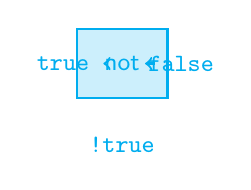
\begin{tikzpicture}[node distance=0.75cm, color=cyan, font=\sffamily\small, thick]

  \node[draw, thick, fill=cyan!20, minimum size=2em, inner sep=1em] (transformer) {not};
  \node (inputs) [left of=transformer] {\texttt{true}};
  \node (outputs) [right of=transformer] {\texttt{false}};
  \node (expression) [below=1em of transformer] {\texttt{!true}};

  \draw[->, thick, shorten >= 1em, shorten <= 0.25em] (inputs) -- (transformer);
  \draw[->, thick, shorten >= 0.25em, shorten <= 0.5em] (transformer) -- (outputs);

\end{tikzpicture}
\\
  \begin{scaletikzpicturetowidth}{\textwidth}
  \begin{tikzpicture}[scale=\tikzscale, node distance=3cm, color=cyan, font=\sffamily\small]

    \node[draw, thick, fill=cyan!20, minimum size=2em, inner sep=1em] (transformer) {not};
    \node (inputs) [left of=transformer] {\texttt{false}};
    \node (outputs) [right of=transformer] {\texttt{true}};
    \node (expression) [below=1em of transformer] {\texttt{!false}};

    \draw[->, thick, shorten >= 1em, shorten <= 0.25em] (inputs) -- (transformer);
    \draw[->, thick, shorten >= 0.25em, shorten <= 0.5em] (transformer) -- (outputs);

  \end{tikzpicture}
\end{scaletikzpicturetowidth}

  \caption{\label{conds:not-fundamental-diagram.tex}The fundamental diagrams for logical \textsf{not} applied to each input.}
\end{figure}

Now you (technically) know everything there is to know about the function logical \textsf{not}. When the input is \texttt{true}, the output \textsf{not} \texttt{true} evaluates to the value \texttt{false}. Likewise, when the input is \texttt{false}, the output \textsf{not} \texttt{false} evaluates to \texttt{true}. Logical \textsf{not} flips Boolean values between \texttt{true} and \texttt{false}.

It is somewhat cumbersome to write out the fundamental diagram for each input value to a function. For functions that operate on a small number of inputs, such as these \textsf{Boolean} operators, it is convenient to collect the inputs and outputs into a table, with one column for each input and another column for an expression of function applied to the inputs, and a final column for the evaluation of the expression.

\begin{figure}[h]
  \ttfamily
  \small
  \color{cyan}
  \begin{tabular}{c  c  c}
    \textsf{Input} & \textsf{Application} & \textsf{Evaluation}\\
    \hline
    true & !true & false\\
    false & !false & true
  \end{tabular}
  \caption{\label{fig:conditionals-logical-not} The truth table for the function logical \textsf{not}.}
\end{figure}

You can create such a table for any function. But when you create this kind of table for combinations of \textsf{Boolean} functions, it gets a special name: a \emph{truth table}. It is extremely easy to get confused when working through the value of a \textsf{Boolean} expression. Even very experienced programmers will get tripped out.\marginnote{Always write things down. Don't try to calculate in your head. You don't get bonus points for doing it in your head.} Truth tables are extremely helpful at making the logic of an expression plain, especially once we start combining operators to make more complicated expressions.

\begin{question}
  Write the pipeline fundamental diagram of the function double \textsf{not} (\texttt{!!}); that is, the function of \textsf{not} applied to the output of \textsf{not}.
\end{question}

\begin{question}
  Write the truth table for double \textsf{not} (\texttt{!!}). \textsc{Hint:} For any input \texttt{x}, \texttt{!!x} evaluate to the same value as \texttt{!(!x)}; that is, the value of \textsf{not} applied to the output of \textsf{not}.
\end{question}

When calculating the value of a boolean expression is very, very helpful to break it down into as many subexpressions as possible. As an example, let's construct the truth table for triple \textsf{not} (\texttt{!!!}). We'd like to be able to write down the answer straight away, but that involves a lot of intermediate calculations. If we tried to keep track of things in our head, it'd be easy to lose track of how many times we've applied \textsf{not}. So, let's expand our table to include all of the intermediate calculations. \marginnote{When working on pipelines with big data, saving intermediate steps becomes even more critical. If the pipeline fails after running for days on a large data set, you'll be happy that you saved intermediate steps instead of starting over at the beginning. Your boss will be happy that you did, too.} It is good and be explicit and write down all of the steps.

Let's make a dummy variable \texttt{x} to be in the input of our expression. In one row, \texttt{x} will be assigned the value \texttt{true}. In the other, \texttt{x} will be assigned the value \texttt{false}. We want to know what the output value \texttt{!!!x} evaluates to. In order to calculate \texttt{!!!x}, we first need to calculate \texttt{!!x}. But to calculate \texttt{!!x}, we first need to calculate \texttt{!x}. But we know how to calculate \texttt{!x}. Let's go!

\begin{figure}[h]
  \ttfamily
  \color{cyan}
  \small
  \begin{tabular}{c c c c}
    x & !x & !!x & !!!x \\
    \hline
    true & false & true & false\\
    false & true & false & true
  \end{tabular}
  \caption{\label{fig:conditional-triple-not-table}The truth table for triple \textsf{not}, with intermediate calculations for subexpressions.}
\end{figure}

\begin{itemize}
  \item boolean data types
  \item comparison operators
  \item transformers can convert one type to another type. that's the transform part! (transformers are stateless?)
  \item equality operators
  \item if statements
  \item scope
  \item running programs
  \item using libraries
  \item command-line arguments
  \item arrays --- multiple values
  \item difference between identity and equality (memory and reference types)
  \item arrays as look-up tables
  \item arrays conditional execution
  \item arrays as finite functions
\end{itemize}


\pagelayout{wide} % No margins
\addpart{Solutions to Problems}
\pagelayout{margin} % Restore margins

\setcounter{chapter}{0}
\renewcommand{\thechapter}{\Alph{chapter}}
\chapter{Introduction}

\ref{question:intro-transformers}. \textbf{TODO}



\backmatter
% The bibliography needs to be compiled with biber using your LaTeX editor, or on the command line with 'biber main' from the template directory
\defbibnote{bibnote}{Here are the references in citation order.\par\bigskip} % Prepend this text to the bibliography
\printbibliography[heading=bibintoc, title=Bibliography, prenote=bibnote] % Add the bibliography heading to the ToC, set the title of the bibliography and output the bibliography note


\end{document}
